%Dokumentinformationen
\newcommand{\titleinfo}{DT2 \_ VHDL - Zusammenfassung}
\newcommand{\authorinfo}{Nicol\'{a}s Rom\'{a}n L\"{u}thold}
\newcommand{\versioninfo}{$Revision V1.1: $ \today}
\newcommand{\verbesserung}{Verbesserungen und Fehler Bitte an: nromanlu@hsr.ch melden}

% standard header
%Schriftgrösse, Layout, Papierformat, Art des Dokumentes
\documentclass[10pt,twoside,a4paper,parskip]{scrartcl}
% fontsize=12pt  Schriftgroesse in 10, 11 oder 12 Punkt
% a4paper        Papierformat ist hier A4
% landscape      Querformat wird natürlich unterstützt ;-)
% parskip        Absatzabstand anstatt Einzüge
% draft          Der Entwurfsmodus deckt Schwächen auf
% {scrartcl}     Die Dokumentenklasse book, report, article
%                oder fürs deutsche scrbook, scrreprt, scrartcl


%Einstellungen der Seitenränder
\usepackage[left=1cm,right=1cm,top=1cm,bottom=1cm,includeheadfoot]{geometry}

% Sprache, Zeichensatz, packages
\usepackage[utf8]{inputenc} % Für automatische erkennung von umluate
\usepackage[ngerman]{babel,varioref} %  Deutsche rechtschribung
\usepackage{amssymb,amsmath,fancybox,graphicx,lastpage,wrapfig,fancyhdr,hyperref}


% für VHDL-code Ausgabe
\usepackage{listings}


%Farben für tabelle
\usepackage{color, colortbl}
\definecolor{Gray}{gray}{0.9}
\definecolor{LightCyan}{rgb}{0.88,1,1}
%\cellcolor{Farbe} für Farben einer Zelle
%\rowcolor{Farbe}  für Farben einer Zeile

%Schriftarten
%http://www.tug.dk/FontCatalogue/arial/
\usepackage[scaled]{uarial}
\renewcommand*\familydefault{\sfdefault} %% Only if the base font of the document is to be sans serif
\usepackage[T1]{fontenc}

%tabularx package
%http://mirror.switch.ch/ftp/mirror/tex/macros/latex/required/tools/tabularx.pdf
%\usepackage{tabularx}
%tabularx: Damit inhalt der Tabelle zentriert ist
%\renewcommand{\tabularxcolumn}[1]{>{\normalsize\centering\arraybackslash}m{#1}}
%aufhebender Befehl
%\def\tabularxcolumn#1{p{#1}}

\usepackage{multirow} % für Tabelle


%pdf info
\hypersetup{pdfauthor={\authorinfo},pdftitle={\titleinfo},colorlinks=false}
\author{\authorinfo}
\title{\titleinfo}

%Kopf- und Fusszeile
\pagestyle{fancy}
\fancyhf{}
%Linien oben und unten
\renewcommand{\headrulewidth}{0.5pt} 
\renewcommand{\footrulewidth}{0.5pt}

\fancyhead[L]{\titleinfo{ }\tiny{(\versioninfo)}}
%Kopfzeile rechts bzw. aussen
\fancyhead[R]{Seite \thepage { }von \pageref{LastPage}}
%Fusszeile links bzw. innen
\fancyfoot[L]{\footnotesize{\authorinfo}}
%Fusszeile mitte bzw. innen
\fancyfoot[C]{\footnotesize{\verbesserung}}
%Fusszeile rechts bzw. ausen
\fancyfoot[R]{\footnotesize{\today}}
 % ./header.tex nicht editieren (Projekt LaTeX-Header benutzen)

%%%%%%%%%%%%%%%%%%%%%%%%%%%%%%%%%%%%%%%%%%%%%%%%%%%%%%%%%%%%%%%%%%%%%%%%%%%%%%%%%%%%%%%%%%%%%%%%
% Neue Befehle und Definitionen                
%%%%%%%%%%%%%%%%%%%%%%%%%%%%%%%%%%%%%%%%%%%%%%%%%%%%%%%%%%%%%%%%%%%%%%%%%%%%%%%%%%%%%%%%%%%%%%%
\definecolor{black}{rgb}{0,0,0}
\definecolor{red}{rgb}{1,0,0}
\definecolor{white}{rgb}{1,1,1}
\definecolor{grey}{rgb}{0.9,0.9,0.9}
\definecolor{gray2}{rgb}{0.5,0.5,0.5}
\definecolor{royalblue}{rgb}{0.15,0.25,0.55}
\definecolor{green}{rgb}{0,0.6,0}

\newcommand{\verweis}[2]{\small{(siehe auch \ref{#1}, #2 (S. \pageref{#1}))}}
\newcommand{\subsubadd}[1]{\textcolor{black}{\mbox{#1}}}

% für VHDL-Code
\lstnewenvironment{VHDL}[1][]
  {\lstset{
  	backgroundcolor=\color{grey},   % choose the background color
    language=VHDL,			
    basicstyle=\footnotesize\ttfamily,
    breaklines=true,
    frame=none,
    columns=flexible,
    keepspaces=true,
    keywordstyle=\color{blue},
    identifierstyle=\color{royalblue},
    commentstyle=\color{green},
    numbers=left,
    numbersep=5pt,
    numberstyle=\tiny\color{gray2},
    rulecolor=\color{black}, 
    stepnumber=1,
    tabsize=4,
  }}{}
  


\begin{document}

%%%%%%%%%%%%%%%%%%%%%%%%%%%%%%%%%%%%%%%%%%%%%%%%%%%%%%%%%%%%%%%%%%%%%%%%%%%%%%%%%%%%%%
% Grundlagen                
%%%%%%%%%%%%%%%%%%%%%%%%%%%%%%%%%%%%%%%%%%%%%%%%%%%%%%%%%%%%%%%%%%%%%%%%%%%%%%%%%%%%%%
\section{Grundlagen Digitaltechnik II}

1975: "The Moore's Low"(Gorden E. Moore, Inter Co-Founder): Anzahl Transistoren auf 1 Chip verdoppelt sich alle 2 Jahre\\

\begin{minipage}{0.5\textwidth}
	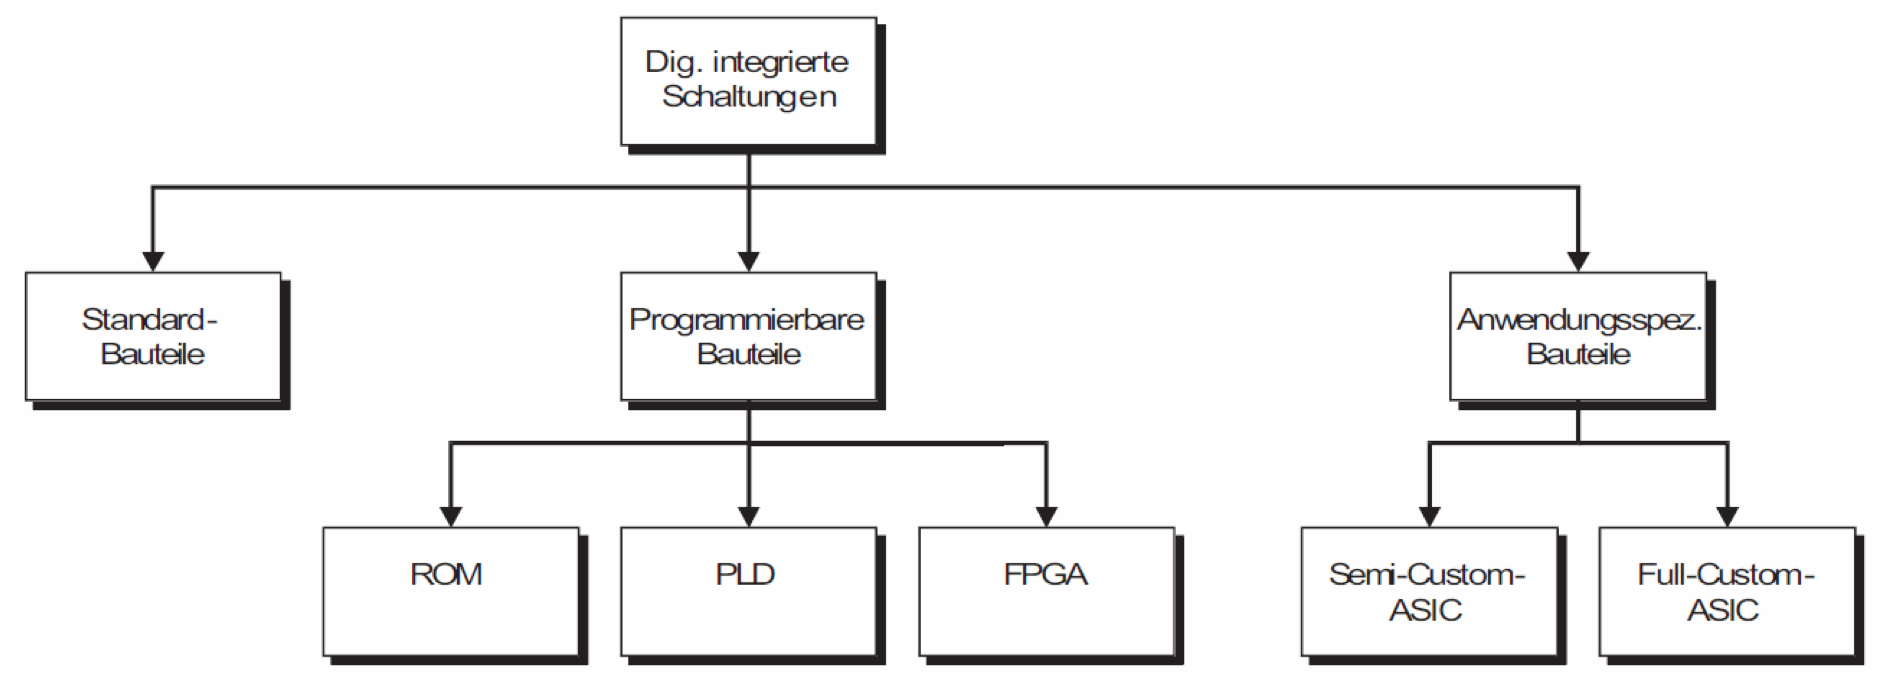
\includegraphics[width=\textwidth]{./bilder/Klassierung}
\end{minipage}
\begin{minipage}[b]{0.5\textwidth}
	\begin{tabular}{l l l}
		SDT-Bauteile 		& Digitale Gates						& AND, OR, ...\\
							& Flipflops 							& \\
		\hline
		Programmier-	 	& ROM {\tiny Read Only Memory}			& PROM {\tiny(one time programmable)}\\
		bare				&										& EPROM {\tiny(eresable with UV)} \\
							&										& EEPROM {\tiny(eresabel with Voltage)}\\
							&										& FLASCH {\tiny (Spezielle EEPROMs)}\\
							\cline{2-3}
							& PDL {\tiny Programable Logic Device}	& PAL {\tiny Programmable Array Logic}\\
							& 										& GAL {\tiny Generic Array Logic} \\
							&										& CPLD {\tiny Complex CLD} \\
							\cline{2-3}
	\end{tabular}
\end{minipage}

\begin{tabular}{l l l l}
	Programmierbare	 		& FPGA {\tiny Field Programmable Gate Array}	& \multicolumn{2}{l}{Im Gegensatz zu PLDs hat es eine regelmässige Strucktur, die in Logik-}\\
	\multicolumn{2}{c}{\multirow{10}{*}{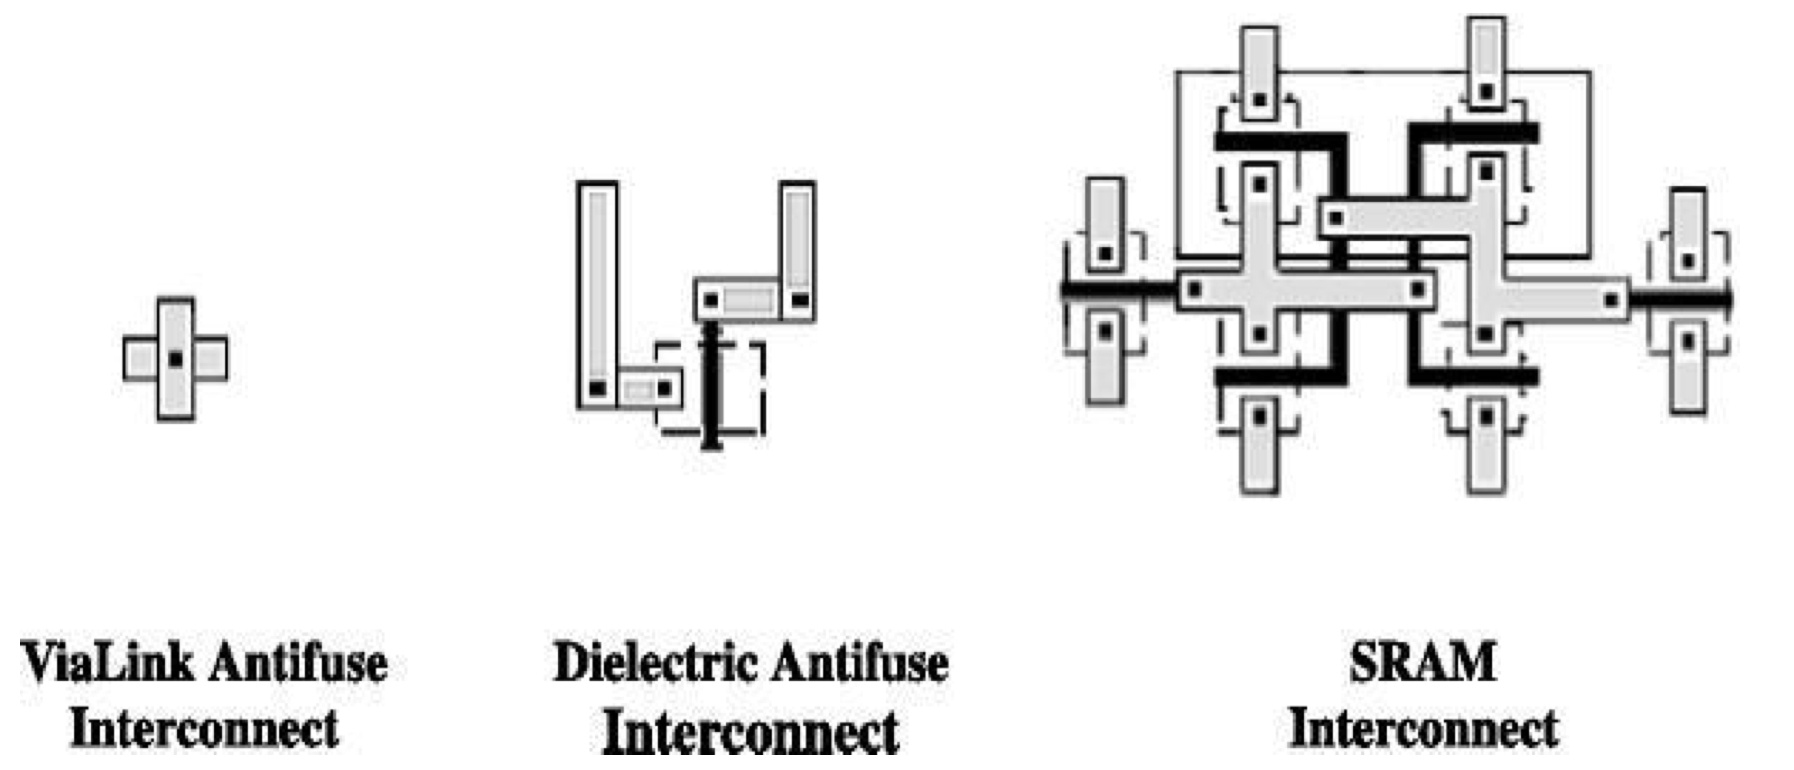
\includegraphics[width=180pt]{./bilder/SRAM}}}	&\multicolumn{2}{l}{ (bei Xilinx CBL) und I/O Blöcke (bei Xilinx IOB)}\\
							&												& \multicolumn{2}{l}{ Man kann Pullup- und Pulldouwnwiderstände hinzuschalten }\\
							&												& \multicolumn{2}{l}{ Schaltpegel sind TTL und CMOS kompatibel}\\
							&		& SRAM - Zelle 							& \multicolumn{1}{|l}{ Antifuse - Technologie}\\
							\cline{3-4}
							&		& Mehrfach Programmierbar				& \multicolumn{1}{|l}{ Verbindung durch Durch-}\\
							&		& Löscht wenn Speisung unterbrochen		& \multicolumn{1}{|l}{ schweissen der Isolation}\\
							&		& hohe Kapazität {\tiny unprogrammiert}	& \multicolumn{1}{|l}{ viel kleiner als SRAM}\\
							&		& geringer Leitwert {\tiny programmiert}& \multicolumn{1}{|l}{ nicht wiederverwendbar}\\
							&		& Stärker verbreitet	 				& \multicolumn{1}{|l}{ sicherer als SRAM}\\
							&		& kann kleine Daten Speichern			& \multicolumn{1}{|l}{ $\rightarrow$ Einsatz im Weltraum}\\
							&		& Startprogramm(e) oft auf PROMS		& \multicolumn{1}{|l}{ }\\
	\hline
	Anwendungsspeziefische	& Semi-Costom									& \multicolumn{2}{l}{Vorgegebenes Grunddesign$\rightarrow$Nutzer macht nur noch Netzmaske}\\
							& 												& \multicolumn{2}{l}{billiger da in Grossen Mengen produziert}\\
							& 												& \multicolumn{2}{l}{kann selten optimal ausgenutzt werden}\\
							\cline{2-4}
							& Full-Custom									& \multicolumn{2}{l}{Spezifische Schaltungen $\rightarrow$ Spezialanfertigung $\rightarrow$ hohe Kosten}\\
							& 												& \multicolumn{2}{l}{Nur in Grossen Mengen rentabel}\\
							& 												& \multicolumn{2}{l}{kann selten optimal ausgenutzt werden}\\
\end{tabular}


%%%%%%%%%%%%%%%%%%%%%%%%%%%%%%%%%%%%%%%%%%%%%%%%%%%%%%%%%%%%%%%%%%%%%%%%%%%%%%%%%%%%%%
% Digitaler Designe-Flow               
%%%%%%%%%%%%%%%%%%%%%%%%%%%%%%%%%%%%%%%%%%%%%%%%%%%%%%%%%%%%%%%%%%%%%%%%%%%%%%%%%%%%%%
\section{Digitaler Designe-Flow}

\begin{minipage}{0.35\textwidth}
	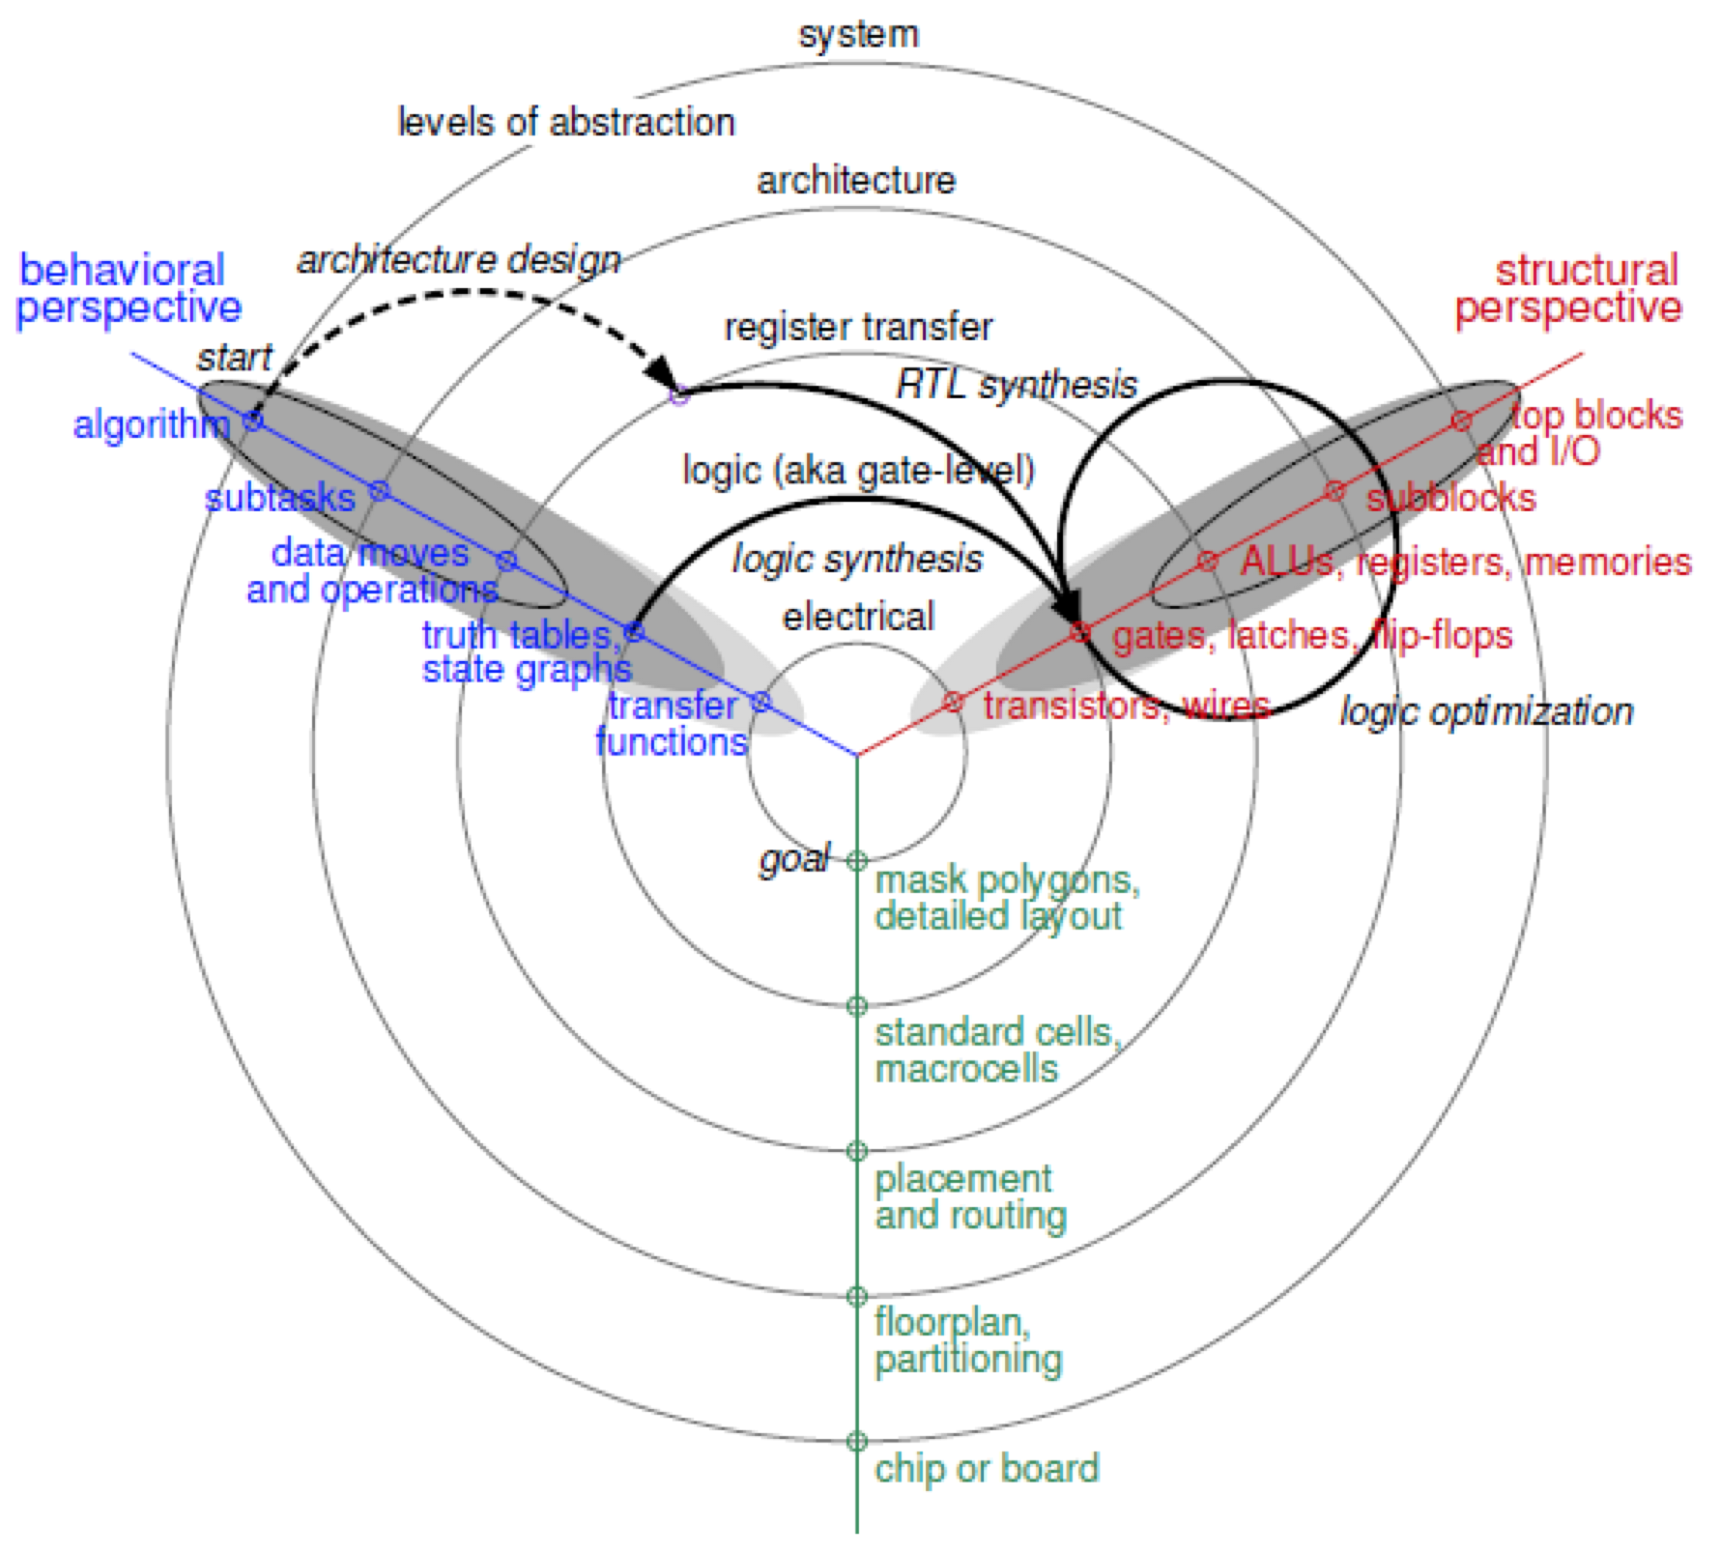
\includegraphics[width=\textwidth]{./bilder/Gajshi}
\end{minipage}
\begin{minipage}{0.6\textwidth}
	\begin{tabular}{l l }
		\multicolumn{2}{l}{\textbf{Y-Model von Gajski}}\\
		1. Verhaltenssicht (blau)		& $\rightarrow$ Wie muss sich das System Verhalten? \\
		2. Struckturelle Sicht (rot)	& $\rightarrow$ Welche elektronische Schaltungen/Baublöcke\\
		3. Physikalische Sicht (grün)	& $\rightarrow$ Wo und wie platziere ich meine Blöcke?\\
	\end{tabular}
	
	\subsection{Desigenprozess}
	\begin{enumerate}
		\item Wichtigste Fragen:
		\begin{itemize}
			\item Welches verhalten will der Kunde
			\item Gewünschte Schnittstellen 
			\item Randbedingungen: Grösse, Kosten, \dots
			\item Soft-, Hardware oder mixed Lösung gewünscht 
			\item Gibt es schon etwas ähnliches auf dem Markt
			\item \dots
		\end{itemize}
	\end{enumerate}
\end{minipage}

\begin{enumerate}
	\setcounter{enumi}{1}
	\item Sobald der Hardwareblock bekannt ist kann man mit dem digitalen Entwurfsprozess starten 
	\item Verhalten werden Verfeinert, Algorithmen zerlegt und in Strukturelle Ebenen übersetzt	
\end{enumerate}

\newpage

\begin{minipage}{.6\textwidth}
	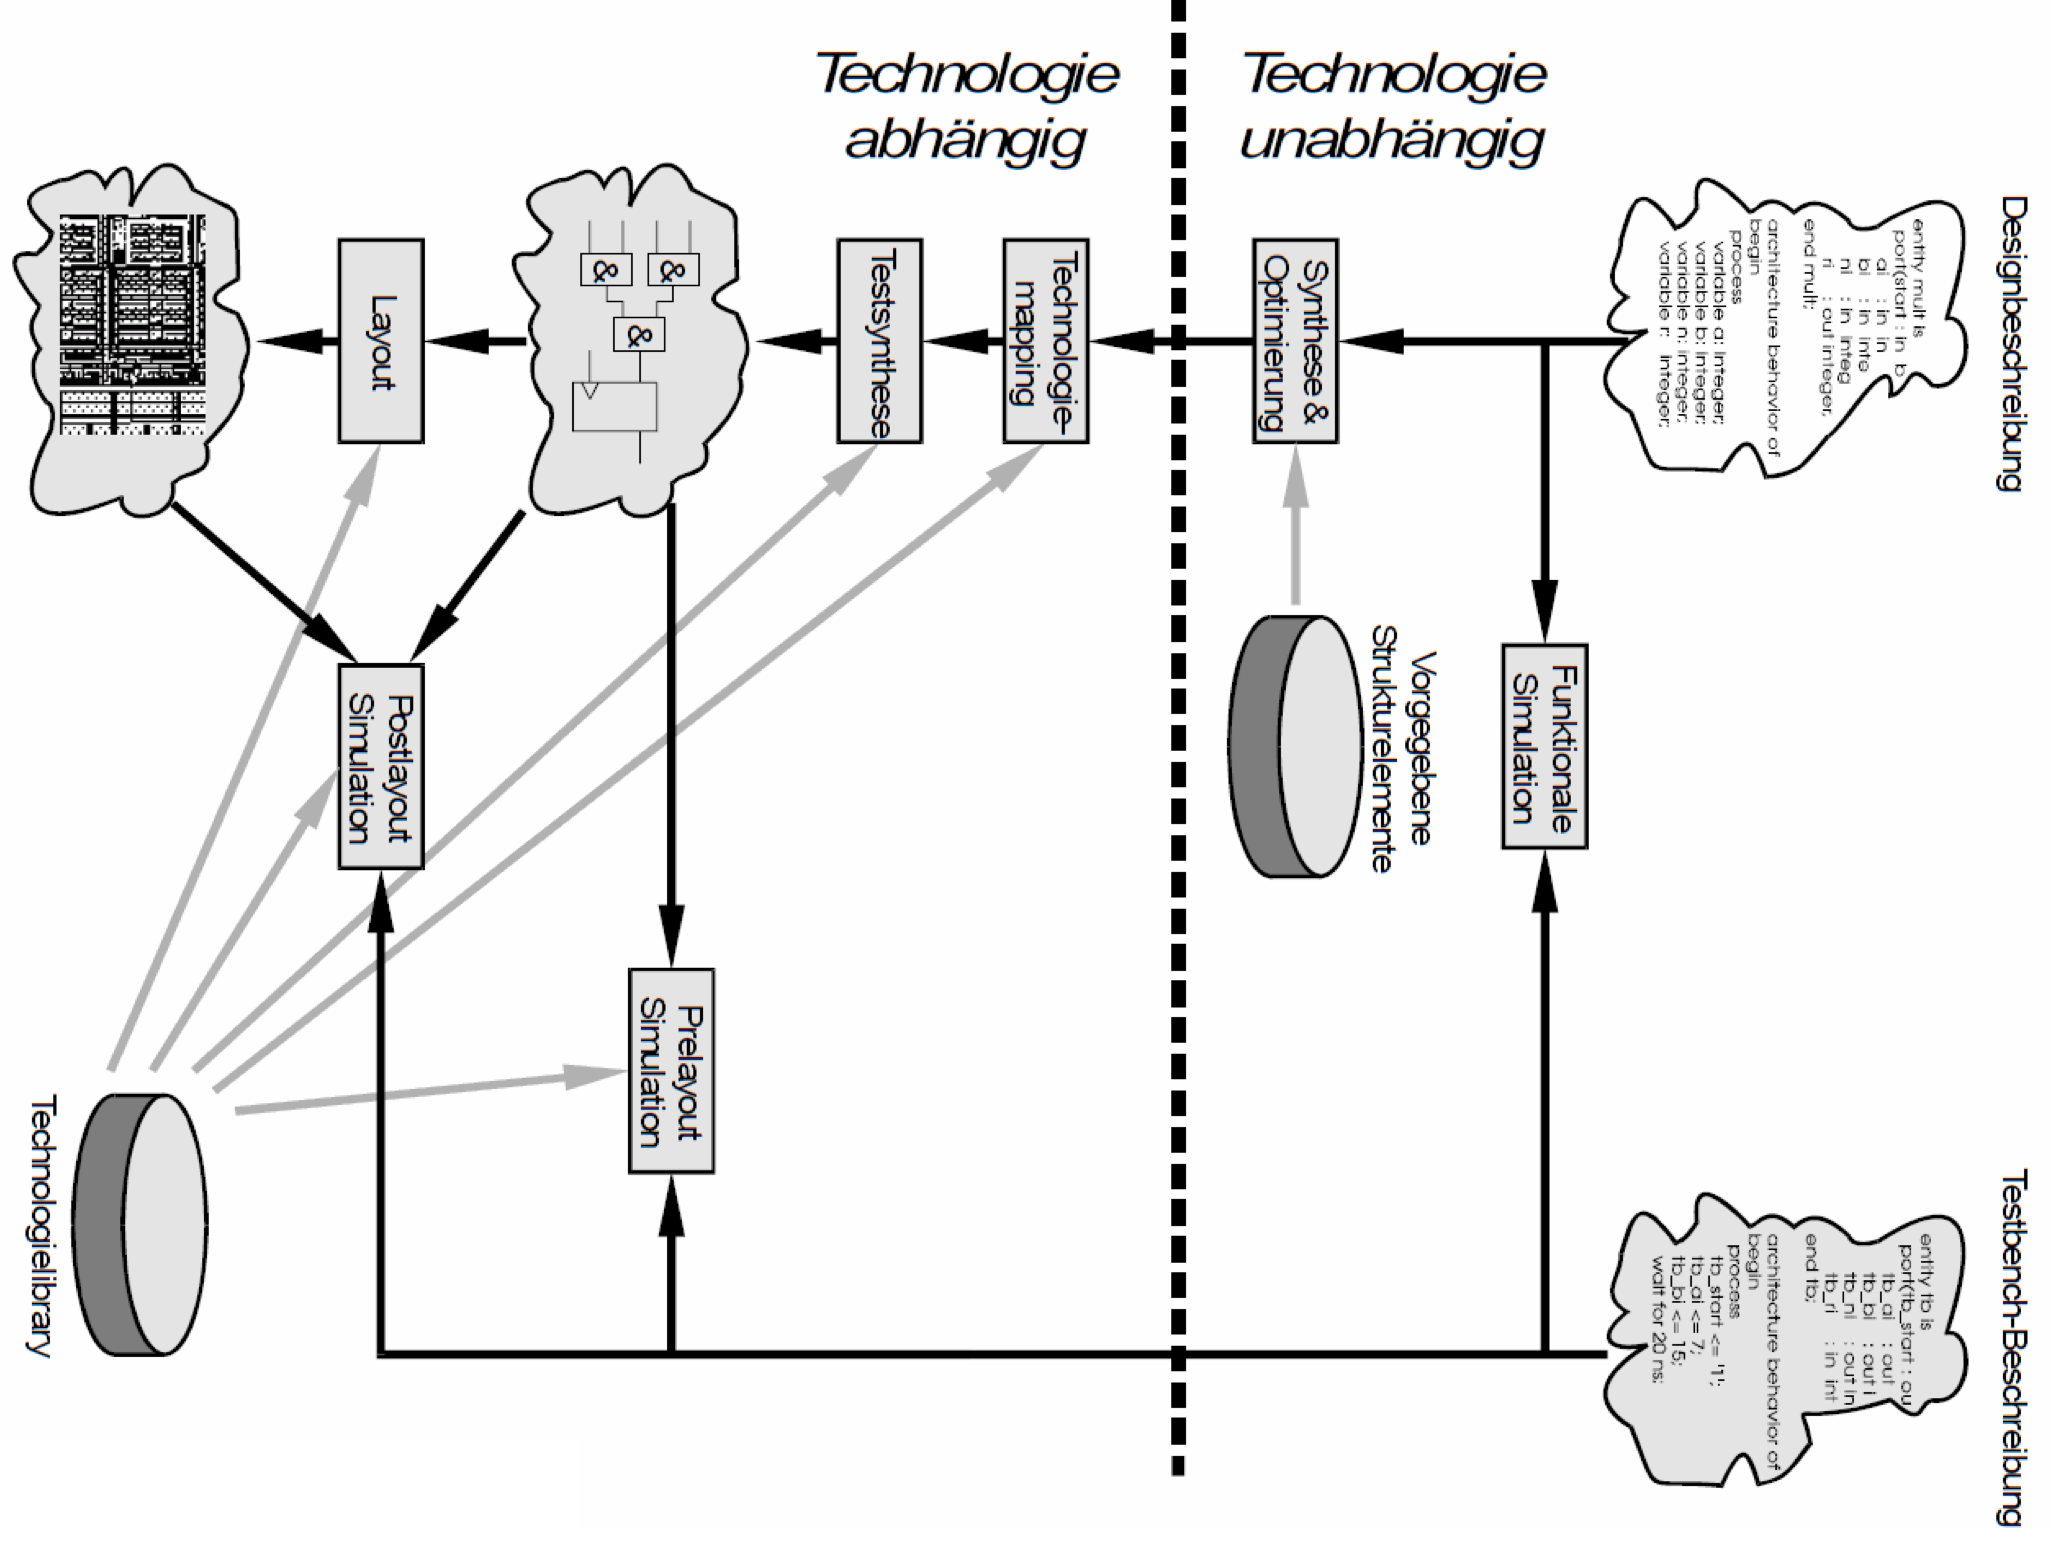
\includegraphics[width=\textwidth]{./bilder/FlowDesigen}
\end{minipage}
\begin{minipage}{.4\textwidth}
	\begin{tabular}{l}
		1. Designbeschreibung\\
		\quad $\rightarrow$ in VHDL \\
		2. Synthese und Optimierung\\
		\quad $\rightarrow$ Übersetzung in generische Netzliste {\tiny(noch kein timing)}\\
		3. Tegnologie Mapping\\
		\quad $\rightarrow$ auf real existierende Baublöcke anpassen\\
		4. Place \& Route\\
		\quad $\rightarrow$ Hardware wird "Programmiert"' (real timing)\\
		5. Simulation \\
		\quad $\rightarrow$ mit Hilfe einer Test-Bench {\tiny(meistens mit einem Zeitdiagramm)}\\
	\end{tabular}
\end{minipage}
%%%%%%%%%%%%%%%%%%%%%%%%%%%%%%%%%%%%%%%%%%%%%%%%%%%%%%%%%%%%%%%%%%%%%%%%%%%%%%%%%%%%%%
% VHDL
%%%%%%%%%%%%%%%%%%%%%%%%%%%%%%%%%%%%%%%%%%%%%%%%%%%%%%%%%%%%%%%%%%%%%%%%%%%%%%%%%%%%%%
\section{VHDL}

\begin{minipage}{0.45\textwidth}
	\begin{tabular}{l}
		\textbf{Überblick}\\
		Kreatives erkennen $\rightarrow$ Mensch\\
		Fleissarbeit $\rightarrow$ CAD Systeme {\tiny (Computer Aided Design)}\\
		"Verilog"' und "'SystemC"' sind alternativen {\tiny (weniger verbreitet)}\\
		Vorteile von VHDL:\\
		\quad $\cdot$ Fokus auf Beschreibung des Verhaltens \\
		\quad $\cdot$ geprägt von kreativen, erfahrungsbasierten Design \\
		\quad $\cdot$ Realisierung von wiederverwendbaren Blöcken \\
	\end{tabular}
\end{minipage}
\begin{minipage}{0.5\textwidth}
	\begin{tabular}{l}
		\textbf{Geschichte}\\
		1980: DoD {\tiny (US Department od Defence)} beauftragt IBM, Intermetrics \\
		\quad und TI eine gemeinsame Hardwaresprache zu definieren\\
		Namen setzt sich von VHSIC {\tiny (Very High Speed Integrated Circuits)} des Dod\\
		\quad und HDL {\tiny (Hardware Description Languege)} zusammen \\
		1987: DoD verzichtet auf das Exklusivrecht \\
		\quad $\rightarrow$ IEEE führt den STD weiter {\tiny (neuster: IEEE 1076.1)} \\
	\end{tabular}
\end{minipage}

\begin{minipage}{0.45\textwidth}
	\begin{tabular}{l}
		\textbf{Charakteristische Elemente}\\
		$\cdot$ Hierarchie und Konnektivität \\
		$\cdot$ Beschreibung und Interpretation \textbf{paralleler} Abläufe \\
		$\cdot$ Beschreibung elektrischer Signale \\
		$\cdot$ Beschreibung des Zeitlichen Verhaltens  \\
		$\cdot$ Parametisierbarkeit von Modellen \\
	\end{tabular}
\end{minipage}
\begin{minipage}{0.32\textwidth}
	\begin{tabular}{l}
		\textbf{Eigenschaften}\\
		$\cdot$ nicht "case sensitiv"  {\tiny Gross- Kleinschreibung}\\
		$\cdot$ Identifier alphanumerisch  \\
		\quad$\cdot$ immer mit Buchstabe beginnen \\
		\quad$\cdot$ keine "\_"' am Ende oder doppelt  \\
		\quad$\cdot$ keine Schlüsselwörter verwenden \\
	\end{tabular}
\end{minipage}
\begin{minipage}{0.2\textwidth}
	\begin{VHDL}
<>  -- identifier
[]  -- Optional Element
{}  -- kann beliebig oft wiederholt werden
	\end{VHDL}
\end{minipage}
%%%%%%%%%%%%%%%%%%%%%%%%%%%%%%%%%%%%%%%%%%%%%%%%%%%%%%%%%%%%%%%%%%%%%%%%%%%%%%%%%%%%%%
% Key Concept I        
%%%%%%%%%%%%%%%%%%%%%%%%%%%%%%%%%%%%%%%%%%%%%%%%%%%%%%%%%%%%%%%%%%%%%%%%%%%%%%%%%%%%%%
\section{Key Concept I \tiny Hierarchie und konektivität}

\subsection{Library}

\begin{minipage}{0.519\textwidth}
	\begin{tabular}{l l}
		\multicolumn{2}{l}{$\cdot$ bereits kompiliert} \\
		\multicolumn{2}{l}{$\cdot$ kann Komponente und/oder Packages enthalten} \\
		$\cdot$ work {\tiny Arbeitsbibliothek} 		& : immer vorhanden {\tiny(wird automatisch generiert)}\\
		$\cdot$ std {\tiny Standartfunktionen} 		& : im IEEE 1076 spezifiziert {\tiny(BIT, INTEGER, ...)}\\
		$\cdot$ ieee {\tiny Praktische Packages}	& : z.B. std\_logic \\
		$\cdot$ PLD, ... {\tiny Hersteller Lib.} 	& : Beschreibung spezifischer Elemente \\
\end{tabular}
\end{minipage}
\begin{minipage}{0.48\textwidth}
	\begin{VHDL}
-- deklaration der Bibliotek
library ieee;	
-- Konstante aus Bibliothek lesen
<variable>:=<library_name>.<consr_name>;
-- Bibliothek sichtbar machen
use <library_name>.<package_name>.<element_name>; -- oder
use <library_name>.all;
	\end{VHDL}
\end{minipage}

\newpage
%--------------------------------------------------------------------------------------
\subsection{Entity}

\begin{minipage}{0.519\textwidth}
	\begin{tabular}{l l}
		$\cdot$ Port 	& : alle digitale Signale, die von aussen sichtbar sind\\
		$\cdot$ Mode	& : in oder out - Ein- Ausgangssignale\\
						& . buffer - zurückführende Ausgangssignale\\
						& . inout - bidirektionale Signale z.B. Busse\\
		$\cdot$ Type 	& : bit, bit\_vector, std\_logic, ... \\
\end{tabular}
\end{minipage}
\begin{minipage}{0.48\textwidth}
	\begin{VHDL}
-- Syntax
entity <ENTITY_NAME> is
	port (
		{<PORT_NAME>: <mode> <type>;}
	);
end <ENTITY_NAME>;	
	\end{VHDL}
\end{minipage}
%--------------------------------------------------------------------------------------
\subsection{Architecture}

\begin{minipage}{0.519\textwidth}
	\begin{tabular}{l l}
		\multicolumn{2}{l}{	mögliche architecture\_names:} \\
		$\cdot$ Behavioral 	& : Verhaltensbeschreibung {\tiny(ähnlich wie Prog.sprachen)}\\
		$\cdot$ Structural	& : Strukturbeschreibung {\tiny(Schaltschema beschrieben)}\\
		$\cdot$ TB 			& : Test-Bench \\
		& \\
		& \\
\end{tabular}


\textbf{Beispiel für Structural}

\end{minipage}
\begin{minipage}{0.48\textwidth}
	\begin{VHDL}
-- Syntax
architecture <architecture_name> of <entity_name> is
	[Type_,Subtype_,Constant_,Signal_,Component_declaration]
begin
	{architecture_body: concurrent actions}
end [architecture_name];	
	\end{VHDL}
\end{minipage}

\begin{minipage}{0.01\textwidth}
	\text{ } %platzhalter
\end{minipage}
\begin{minipage}{0.48\textwidth}
	\begin{VHDL}
-- Deklaration
component <component_name>
	port (
		{port_name: <port_mode><port_type>});
end component;

signal <internal_signal_name>: <sygnal_type>;	
	\end{VHDL}
\end{minipage}
\begin{minipage}{0.02\textwidth}
	\text{ } %platzhalter
\end{minipage}
\begin{minipage}{0.48\textwidth}
	\begin{VHDL}
-- Initialisierung
<instance_name>: <component_name>
	port map (	-- explizit
		<instance_port_name> => <external_signal_name>,
		<instance_port2_name> => <external_signal2_name>);	
		-- or implizit
		(<external_signal_name>, <external_signal2_name>)
	\end{VHDL}
\end{minipage}
%%%%%%%%%%%%%%%%%%%%%%%%%%%%%%%%%%%%%%%%%%%%%%%%%%%%%%%%%%%%%%%%%%%%%%%%%%%%%%%%%%%%%%
% Key Concept II       
%%%%%%%%%%%%%%%%%%%%%%%%%%%%%%%%%%%%%%%%%%%%%%%%%%%%%%%%%%%%%%%%%%%%%%%%%%%%%%%%%%%%%%
\section{Key Concept II \tiny Nebenläufige Prozesse und Prozessiteration}

\subsection{Signale}

\begin{minipage}{0.01\textwidth}
	\text{ } %platzhalter
\end{minipage}
\begin{minipage}{0.48\textwidth}
	\begin{VHDL}
--  Definition 
signal <signal_name1> {,<signal_name2>}: <singal_type> [:= initial_value]
-- Std zuweisung
y <= x;
-- Unbedingte Signalzuweisung 
[label:] <signal_name> <= Expression {, Exression};
Y <= '1'; ["100101";] [A and B;]	-- Beispiele
	\end{VHDL}
\end{minipage}
\begin{minipage}{0.02\textwidth}
	\text{ } %platzhalter
\end{minipage}
\begin{minipage}{0.48\textwidth}
	\begin{VHDL}
-- Selektive Signalzuweisung
[label:] with <select_signal> select
	<dest_sig> <= 	{surce_sig_1 when select_value_1,}
					source_sig_n when others;
-- Bedingte Signalzuweisung
[label:] <dest_sig> <=	{expr_1 when condition_1 else}
						expr_n
	\end{VHDL}
\end{minipage}

\subsection{Nebenläufigkeit Prozesse}

\begin{minipage}{0.01\textwidth}
	\text{ } %platzhalter
\end{minipage}
\begin{minipage}{0.35\textwidth}
	\begin{VHDL}
--  Definition 
[<label:] process [(<Sensitivitaetsliste>)] -- falls keine, wait nicht vergessen
	<Deklarationsteil> -- Prozess intern
begin 
	{<sequentielle Anweisungen>}
end process [<lable>];
-- nur Variabeln im Prozesses aenderbar Bsp.
variable <var_name>: <type> [ := expr]; 
	\end{VHDL}
\end{minipage}
\begin{minipage}{0.02\textwidth}
	\text{ } %platzhalter
\end{minipage}
\begin{minipage}{0.26\textwidth}
	\begin{VHDL}
-- sequenzielle Anweisungen - if
if condition_a then 
	{sequential statements};
{elsif condition_b then
	{sequential statements};}
else 
	{sequential statments};
end if;

	\end{VHDL}
\end{minipage}
\begin{minipage}{0.02\textwidth}
	\text{ } %platzhalter
\end{minipage}
\begin{minipage}{0.32\textwidth}
	\begin{VHDL}
-- case
case expression is 
	when choice_1 	=> {sequential statement};
	{when choice_n	=> {sequential statement};}
	when others	  	=> {sequential statement};
end case;
	\end{VHDL}
\end{minipage}


\subsection{Sequentielle Schaltung}

\begin{minipage}{.5\textwidth}
	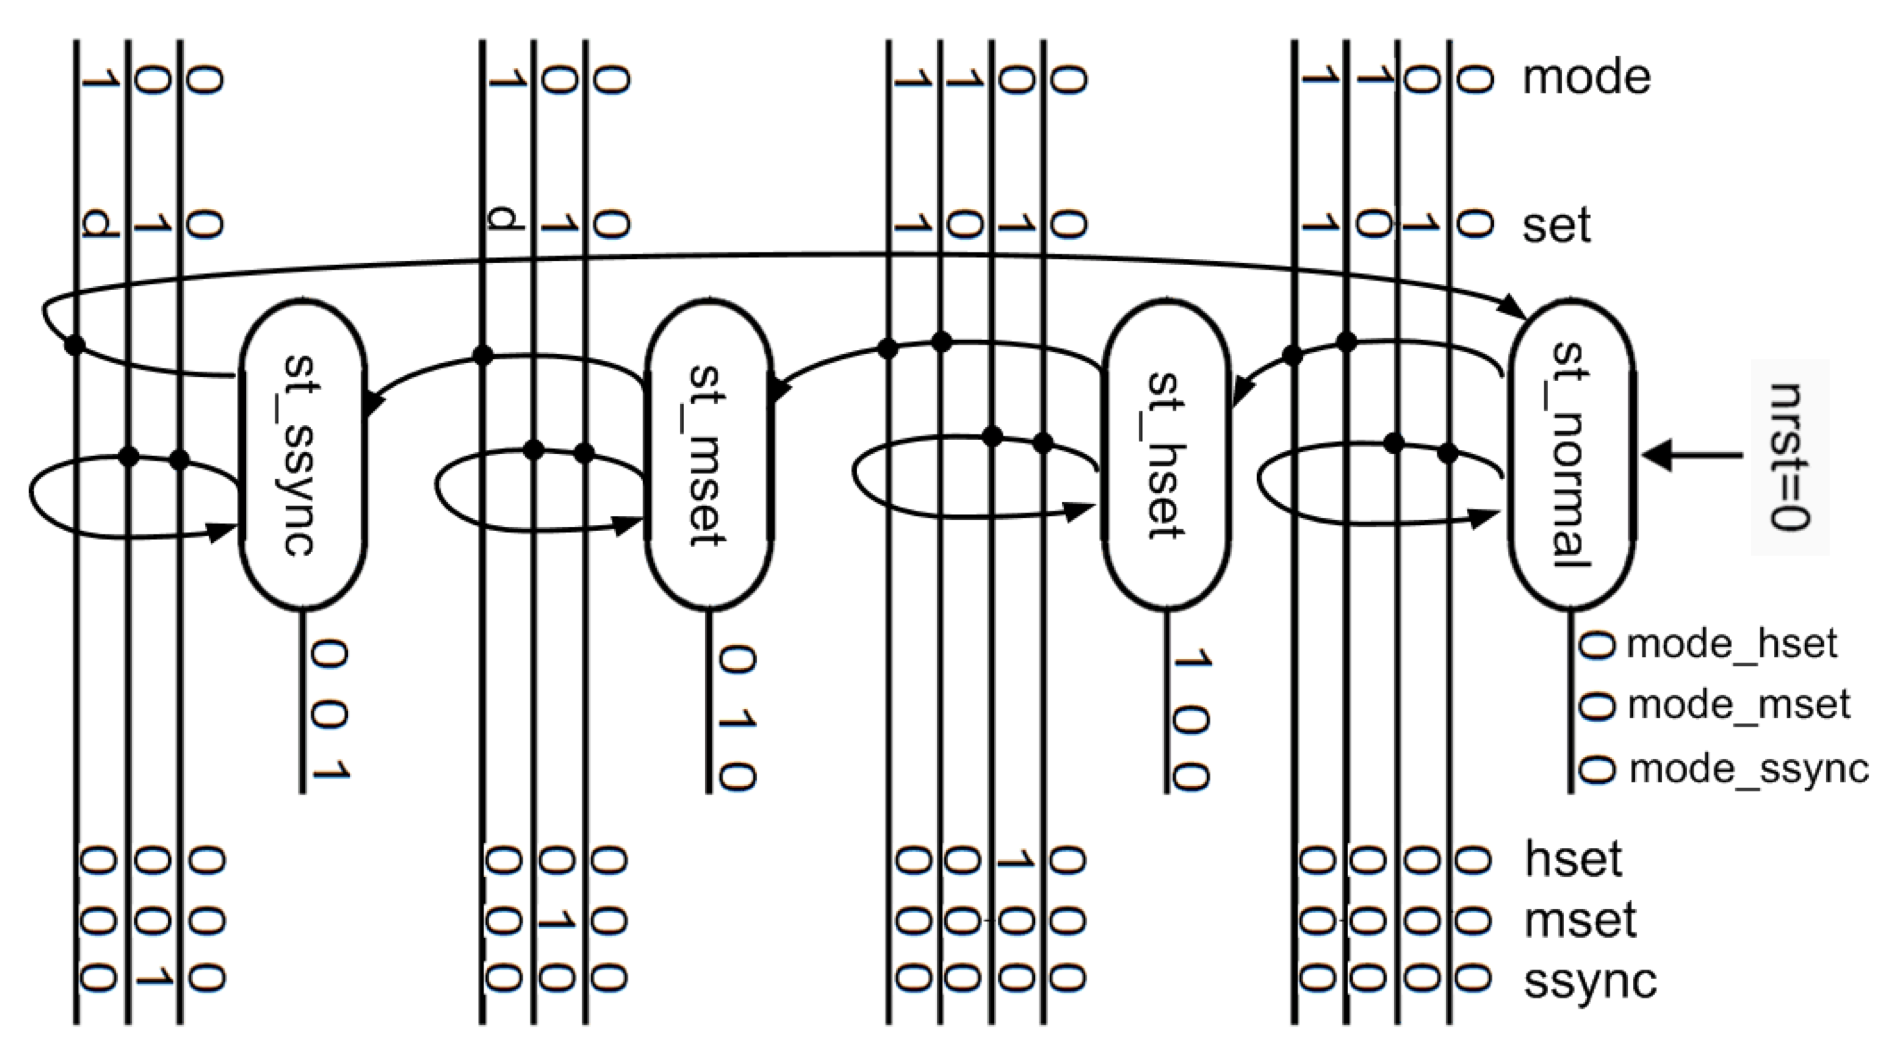
\includegraphics[width=\textwidth]{./bilder/ZDiagramm}
\end{minipage}
\begin{minipage}{0.02\textwidth}
	\text{ } %platzhalter
\end{minipage}
\begin{minipage}{.48\textwidth}
	$\cdot$ FSM ähnliche Zustände wie Z-Diagramm\\
	$\cdot$ empfohlen die Übergänge mit einem CLK zu lösen
	\begin{VHDL}
if CLK'event and (CLK = '1') then {} -- pos falnke ('0' neg) \end{VHDL}

	$\cdot$ Signale in synchronem Prozess auf linker Seite -> FF{\tiny Flip-Flop} \\
	$\cdot$ in Sensitivitätsliste nur CLK (und RST)\\
	$\cdot$ if Anweisungen mit CLK immer am Schluss des Prozesses\\
	$\cdot$ Aufzählungstyp (z.B. für Prozessname) {\tiny  Anzahl Bits kann auch defieniert werden}
	\begin{VHDL}
type <enum_type_name> is (type_element{, type_element});	\end{VHDL}
	$\cdot$ hinterlegte Bits für Aufzählungstyp selber bestimmen
	\begin{VHDL}
attribute <ENUM> : <ENUM_type>;	-- ENUM encoding
attribute <ENUM> of	<aufz_type> : type is expression
subtype <aufz_type> is <const_type>; -- constant encoding
constant <aufz_type_element> : <aufz_type> := expression  \end{VHDL}
\end{minipage}

\subsection{Endliche Z-Maschinen}

\begin{minipage}{.6\textwidth}
	\begin{VHDL}
-- Prozess G = next_state_logic: Kombinatorischer Prozess
	next_state_logic: process (INP, present_state)
	begin 
		{Kombinatorische Anweisungen} -- Bestimmung des next_state
	end process;
	
-- Prozess Z = state_register:
	state_register: process (CLK, RST)
	begin 
		{Sequentielle Anweisungen} -- Aktualisiert bei CLK den present_state
	end process;
 
-- Prozess F = Output_Logic: 1. Mealy
	output_logic: process (INP, present_state)
	begin
		{output_bestimmung} -- Ausgang von IMP und present_state abhaengig
	end process
-- 2. Moore
	output_logic: process (present_state)
	begin
		{output_bestimmung} -- Ausgang nur vom present_state abhaengig
	end process
-- 3. Medwedjew
	output_logic: OUP <= present_state;
	\end{VHDL}
\end{minipage}
\begin{minipage}{.4\textwidth}
	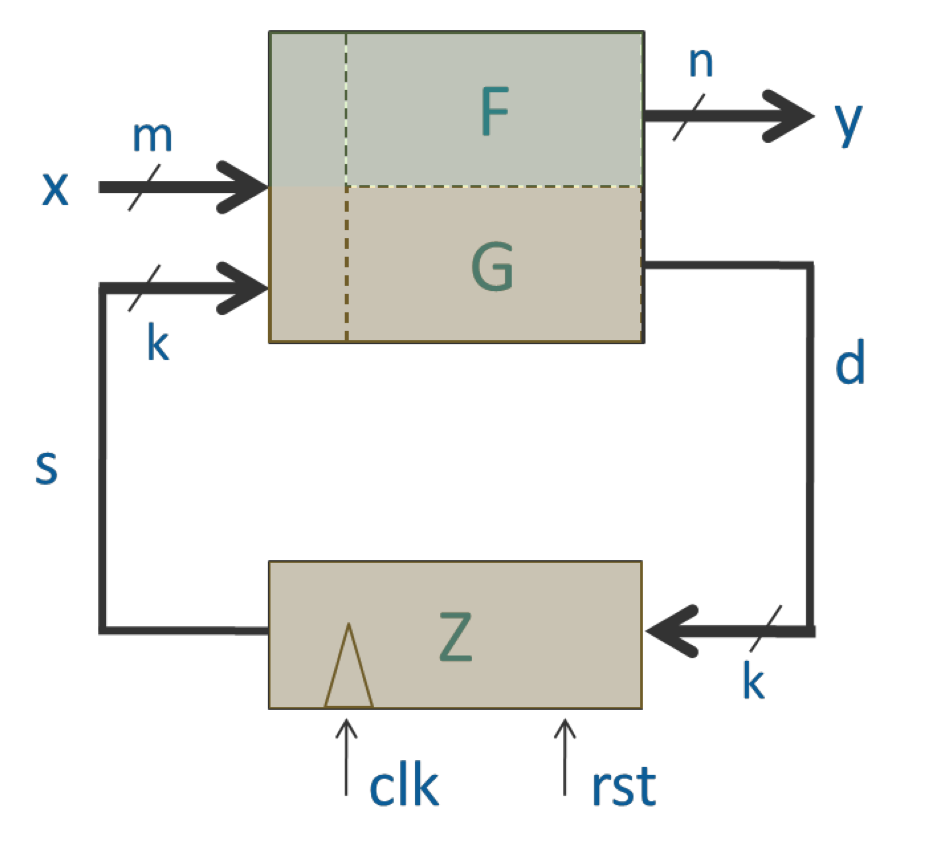
\includegraphics[width=\textwidth]{./bilder/ZMaschiene}
\end{minipage}

%%%%%%%%%%%%%%%%%%%%%%%%%%%%%%%%%%%%%%%%%%%%%%%%%%%%%%%%%%%%%%%%%%%%%%%%%%%%%%%%%%%%%%
% Key Concept III       
%%%%%%%%%%%%%%%%%%%%%%%%%%%%%%%%%%%%%%%%%%%%%%%%%%%%%%%%%%%%%%%%%%%%%%%%%%%%%%%%%%%%%%
\section{Key Concept III \tiny Diskreter Ersatz für elektrische Signale}

\begin{tabular}{l|l}
	\multicolumn{2}{l}{\textbf{use.std\_logic\_1164.all} enthält folgende 2 Datentype}  \\
	std\_logic														& std\_ulogic \\
	\hline
	$\cdot$ solved logic											& $\cdot$ unsolved logic\\
	$\cdot$ erlaubt mehrere Treiber an einem Signal. Siehe Tabelle	& $\cdot$ erlaubt auch mehrere Treiber es darf aber nur einer aktiv sein \\
	$\rightarrow$ Kurzschluss Gefahr!								& $\rightarrow$ Kein Kurzschluss möglich  \\
	$\cdot$ Subklasse von std\_ulogic								& $\cdot$ erkennt in der Sim. nicht initialisierte Signale {\tiny bezeichnet sie als "`U"'}\\
	$\cdot$ erlaubt Modellierung von Schwachen Signalen (L und H)	& $\cdot$ erlaubt Modellierung von Schwachen Signalen (L und H)\\
	$\cdot$ erlaubt DONT'CARES (Signalwert '-')						& $\cdot$ erlaubt DONT'CARES (Signalwert '-')	\\
	$\cdot$ erlaubt bidirektionale Busse							& $\cdot$ nur einfache Busse erlaubt\\
	$\cdot$ grosser Simulationsaufwand								& $\cdot$ kleinerer Simulationsaufwand als std\_logic\\
	$\cdot$ Vektorform: std\_logic\_vector							& $\cdot$ Vektorform: std\_ulogic\_vector\\
\end{tabular}

\begin{minipage}{0.5\textwidth}
	\subsection{Busse}
	\begin{tabular}{l}
		$\cdot$ Master bestimmt welcher Slave spricht \\
		$\cdot$ Alle Teilnehmer (Slaves) können den Bus jederzeit abhören \\
		$\cdot$ Unaktive Treiber auf "`Z"' um den Datenverkehr nicht zu stören \\
		$\cdot$ Beschreibung des Zeitlichen Verhaltens  \\
		$\cdot$ Parametisierbarkeit von Modellen \\
	\end{tabular}
	\begin{minipage}{0.5\textwidth}
		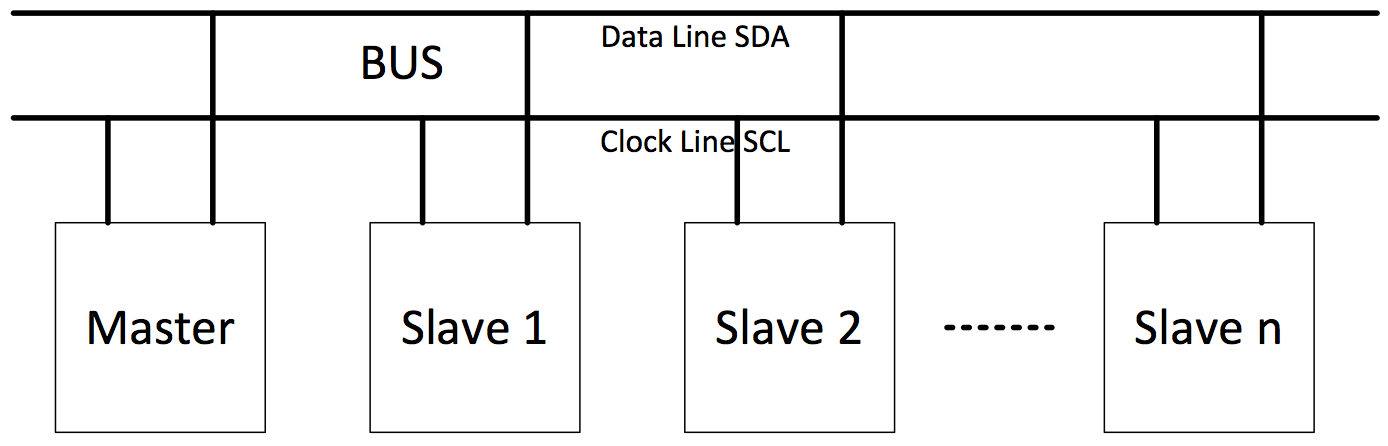
\includegraphics[width=\textwidth]{./bilder/Bus1}
	\end{minipage}
	\begin{minipage}{0.4\textwidth}
		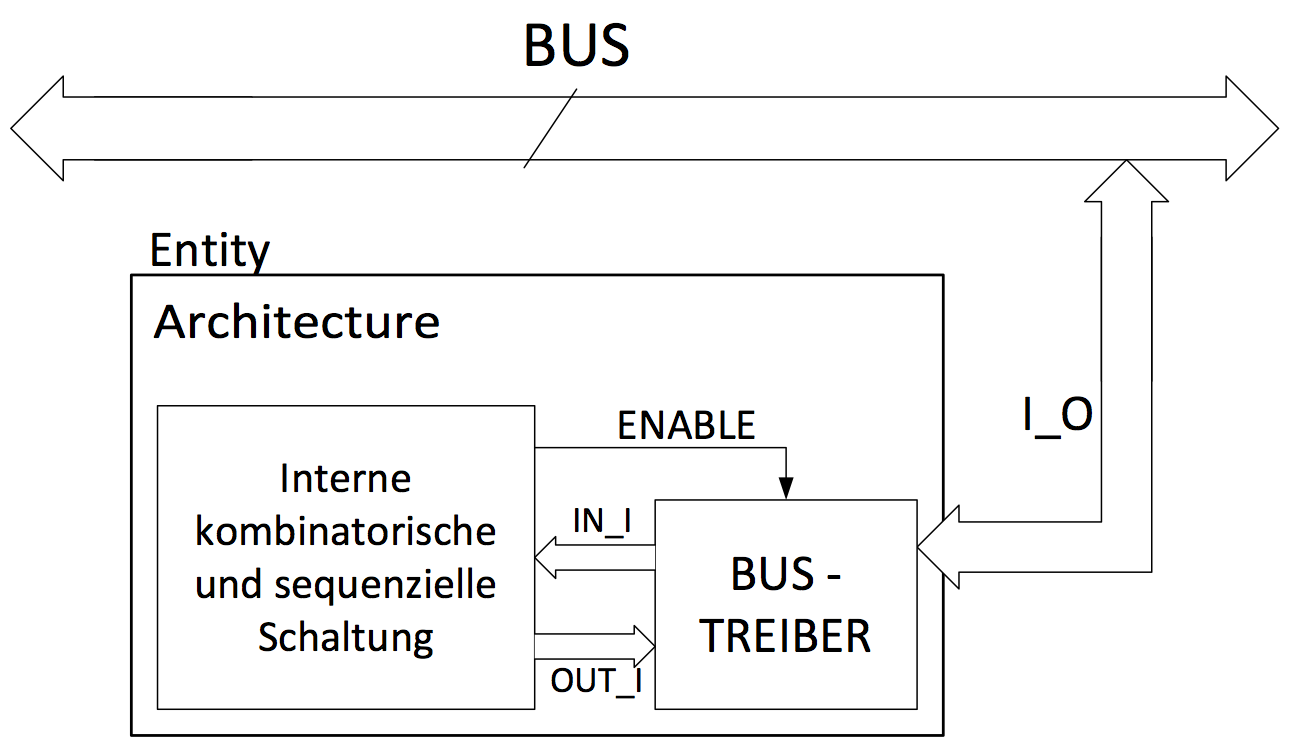
\includegraphics[width=\textwidth]{./bilder/Bus2}
	\end{minipage}
	\subsection{Codierungsempfehlung}
\end{minipage}
\begin{minipage}{0.5\textwidth}
	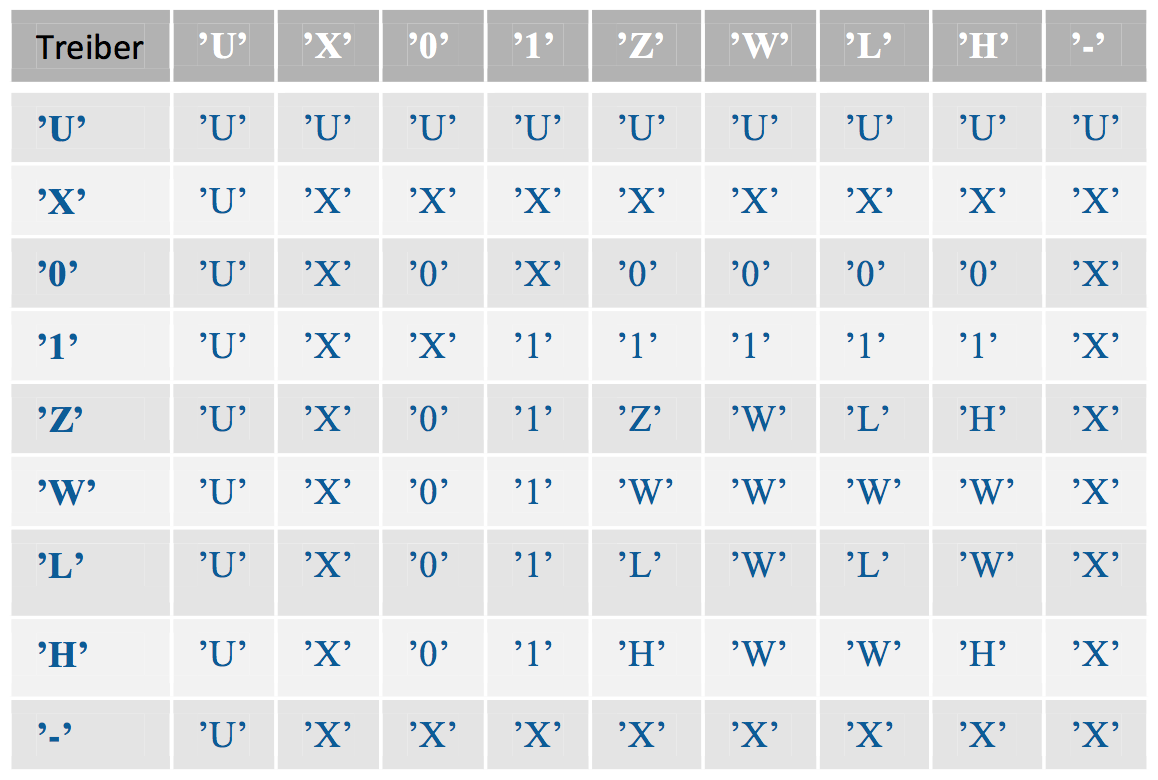
\includegraphics[width=\textwidth]{./bilder/Treiber}
\end{minipage}

Falls immer möglich (in den Übungen) std\_ulogic verwenden, obwohl in der Praxis std\_logic verbreitet ist. std\_logic ist eine Unterklasse von std\_ulogic und damit kompatibel, was aber nicht andersrum gilt! std\_logic\_vektor ist trotz Unterklasse erst seit 2008 mit std\_ulogic\_vektor kompatibel (dieser neuer STD ist noch nicht weit verbereitet!).
%%%%%%%%%%%%%%%%%%%%%%%%%%%%%%%%%%%%%%%%%%%%%%%%%%%%%%%%%%%%%%%%%%%%%%%%%%%%%%%%%%%%%%
% Arithmetick und Datentypen
%%%%%%%%%%%%%%%%%%%%%%%%%%%%%%%%%%%%%%%%%%%%%%%%%%%%%%%%%%%%%%%%%%%%%%%%%%%%%%%%%%%%%%
\section{Arithmetick und Datentypen}

\begin{minipage}{0.4\textwidth}
	\begin{tabular}{l|l}
		\multicolumn{2}{l}{\textbf{Logische Operatoren}}  \\
		\multicolumn{2}{l}{für bit, bit\_vector, std\_(u)logic, std\_(u)logic\_vector }\\
		mit STD Library		& mit ieee.numeric\_std {\tiny ieee.numeric\_bit}\\
		\hline
		$\cdot$ and, nand	& $\cdot$ + ,-\\
		$\cdot$ or, nor		& $\cdot$ signed, unsigned \\
		$\cdot$ xor, xnor	& $\cdot$ abs, mod, rem\\
		$\cdot$ not			& $\cdot$ *, /, **\\
	\end{tabular}
	
	\subsection{Datentypen}
	
	\begin{VHDL}
-- Aufzaelungstyp
type <my_type> is ({my_value_1,} my_value_n);
type traffic_light is (rot, bruen, orange);-- Bsp.
-- Physikalische Typen
tyle PHYS_NAME is range RANGE_OF_VALUES
units
	BASE_UNIT;
	{MULTIPLES;}
end units
tyle CAPACITANCE is range 0 to 1E30 -- Bsp
units
	pF;
	nF = 1000 pF;
	uF = 1000 nF;
end units
-- Arraytyp
type ARRAY_NAME is array
	(UPPER_LIM downto LOWER_LIM) of BASE_TYPE;
type VECTOR_1 is array  -- Bsp
	(9 downto 0) of integer;
	\end{VHDL}
	
\end{minipage}
\begin{minipage}{0.6\textwidth}
	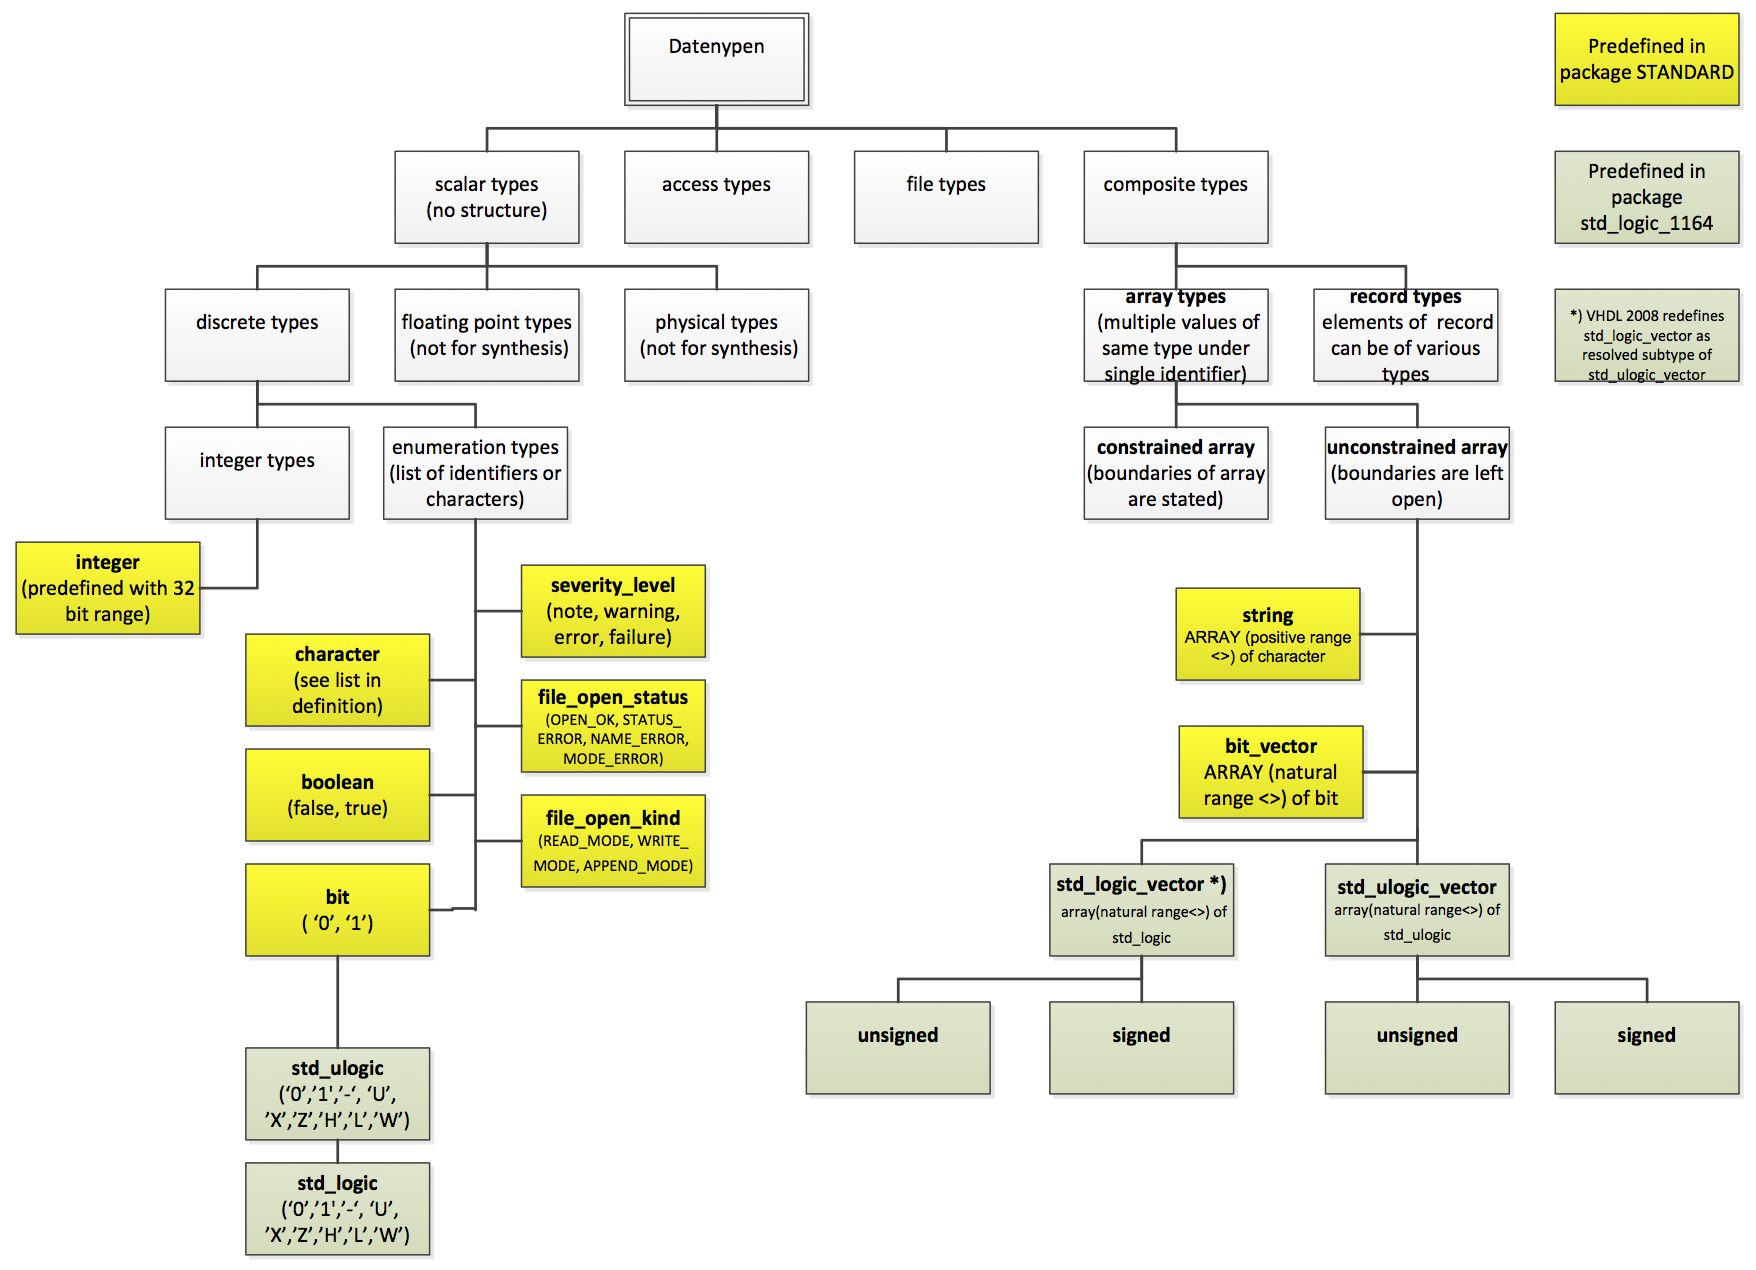
\includegraphics[width=\textwidth]{./bilder/Datentypen}
	
	\begin{minipage}{0.02\textwidth}
		\text{ } %platzhalter
	\end{minipage}
	\begin{minipage}{0.72\textwidth}
		\begin{VHDL}
	-- Resize
	function RESIZE (ARG: signed; NEW_SIZE: natural)
	return signed;
	y <= resize(A,y'length) + resize(B,y'length);
	-- Type_cast
	target_signal <= target_type (source_signal);
	-- Type_convercion
	target_signal <= to_<target_type> (source_signal);	\end{VHDL}	
	\end{minipage}
	\begin{minipage}{0.02\textwidth}
		\text{ } %platzhalter
	\end{minipage}
	\begin{minipage}{0.18\textwidth}
		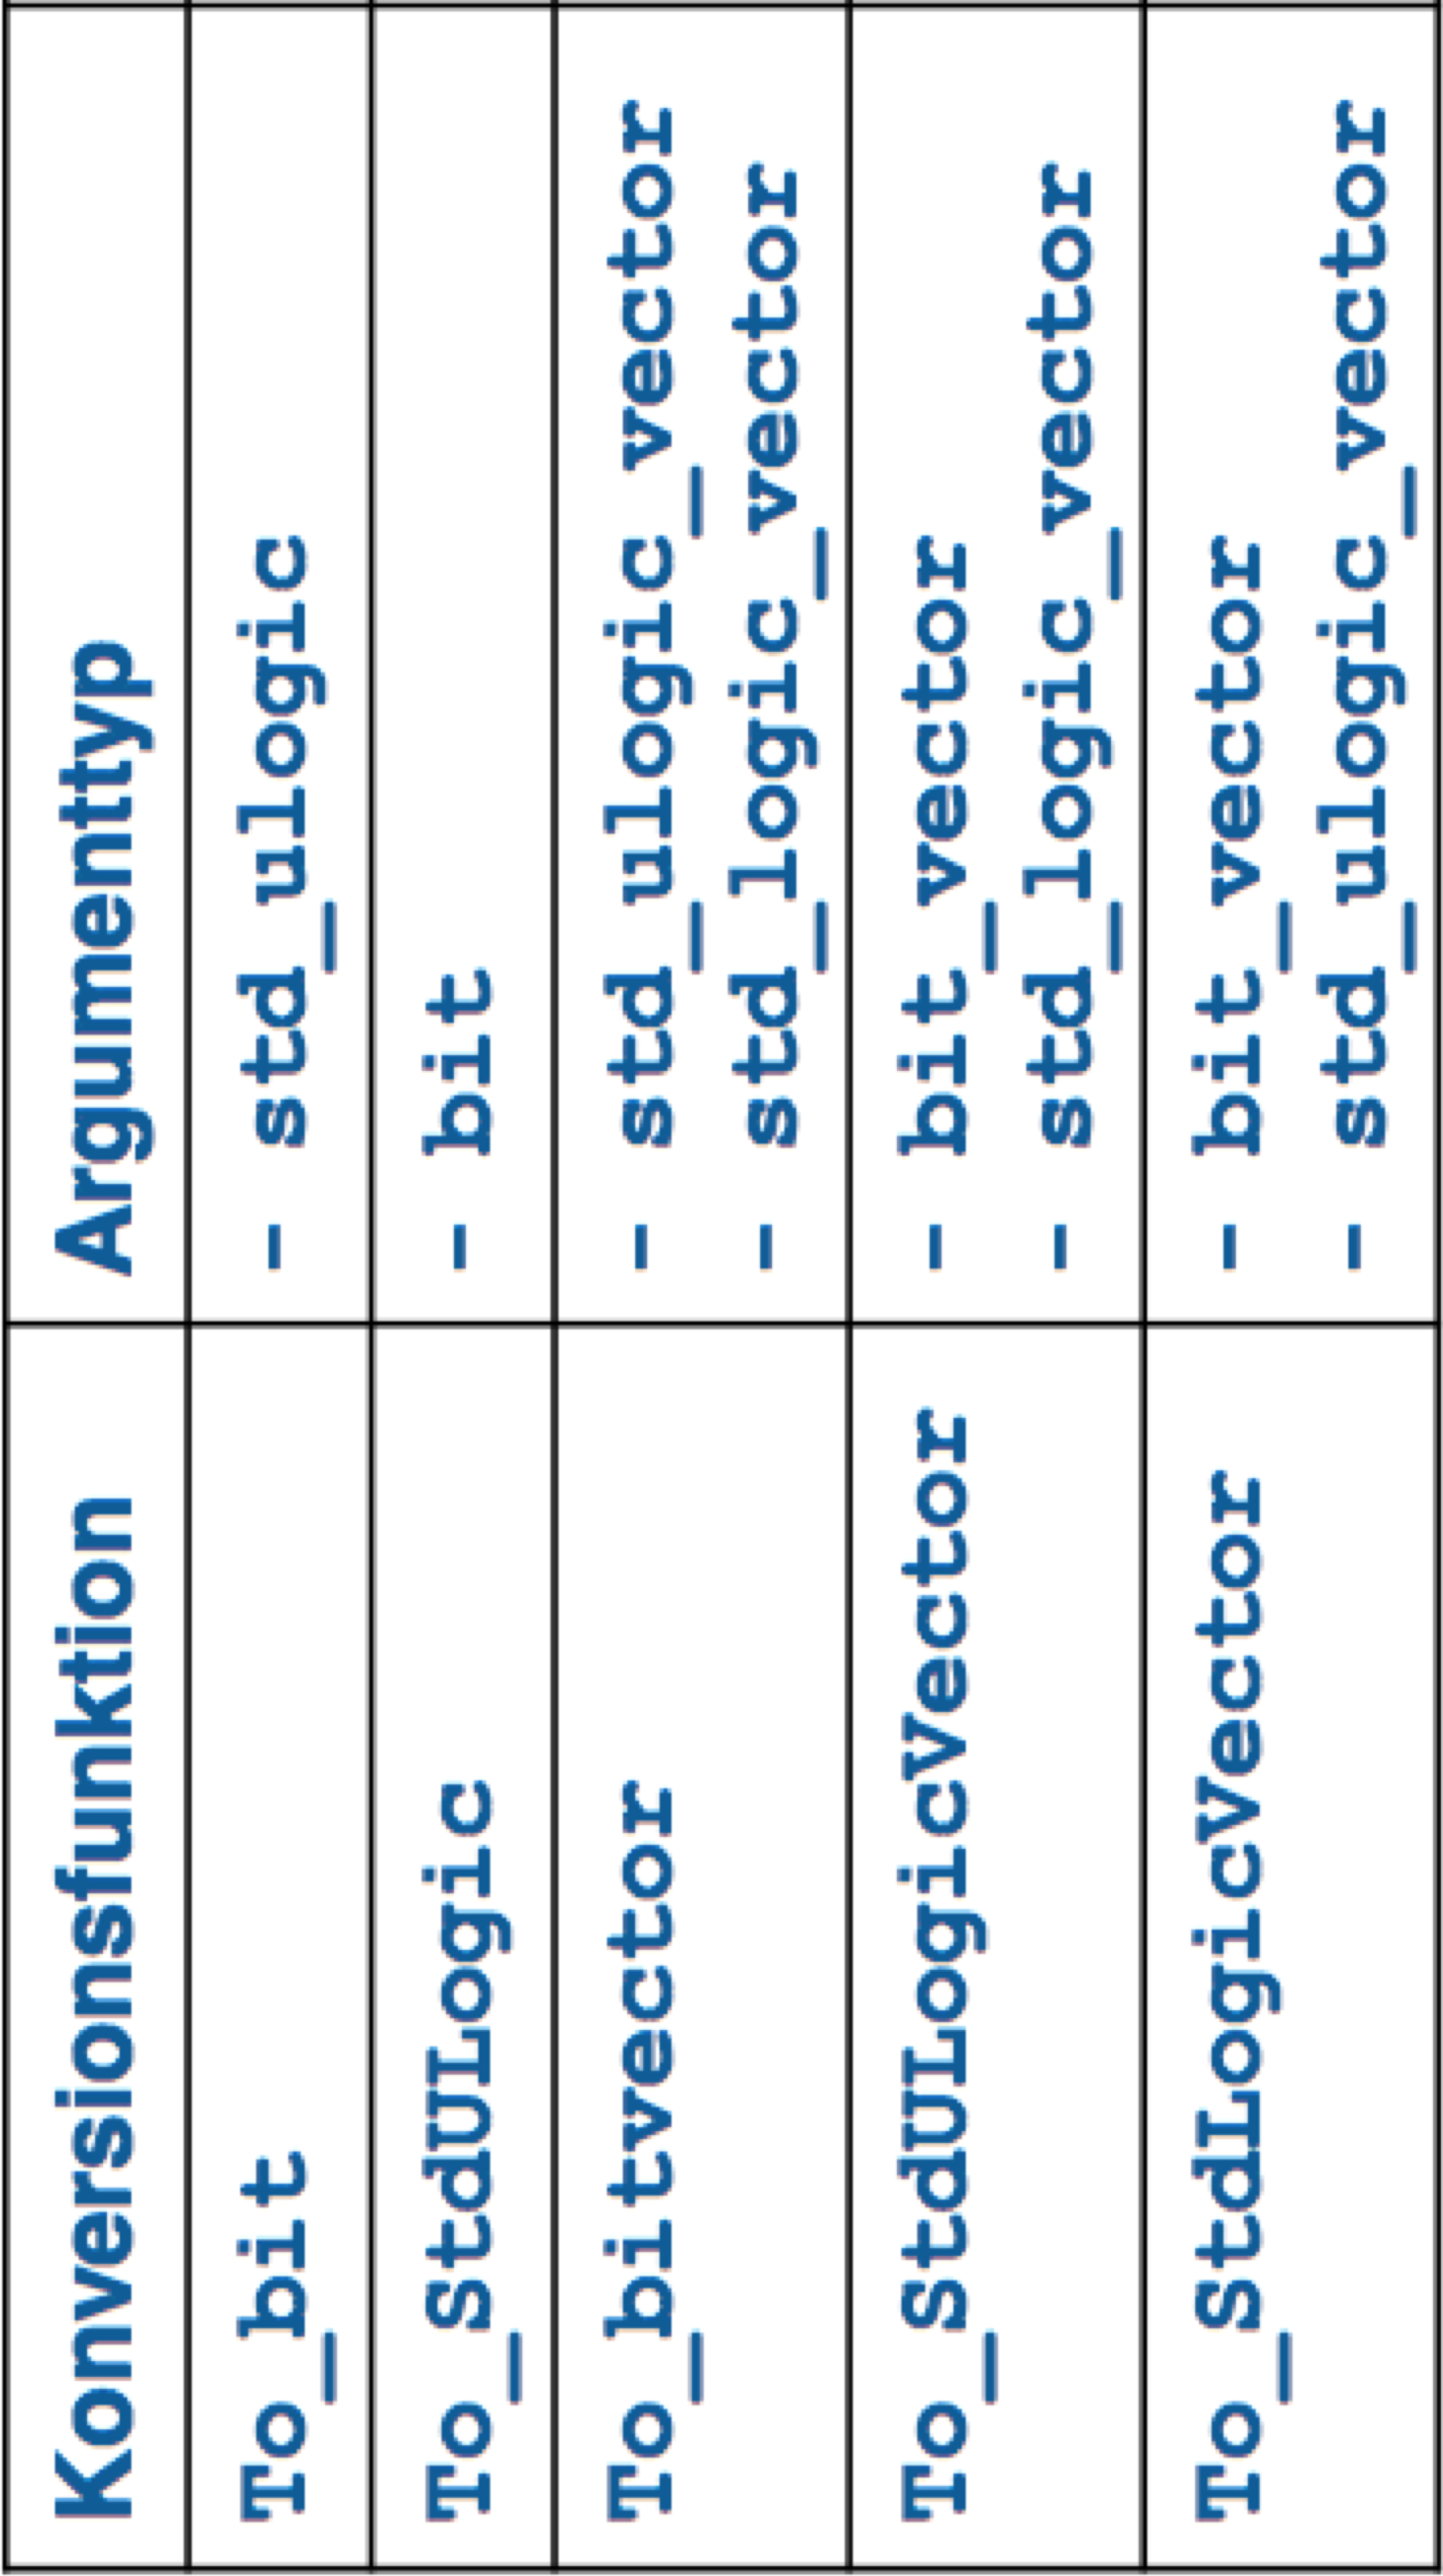
\includegraphics[width=\textwidth]{./bilder/Konversion}
	\end{minipage}
\end{minipage}

%%%%%%%%%%%%%%%%%%%%%%%%%%%%%%%%%%%%%%%%%%%%%%%%%%%%%%%%%%%%%%%%%%%%%%%%%%%%%%%%%%%%%%
% Key Concept IV       
%%%%%%%%%%%%%%%%%%%%%%%%%%%%%%%%%%%%%%%%%%%%%%%%%%%%%%%%%%%%%%%%%%%%%%%%%%%%%%%%%%%%%%

\newpage

\section{Key Concept IV \tiny Zeitliche Darstellung bei Simulation}

\begin{minipage}{0.6\textwidth}
	\begin{tabular}{l}
		$\cdot$ Die Simulation / Funktionstest wird mit Hilfe einer Test-Banch gemacht \\
		$\cdot$ Die Test-Banch sollte Wiederverwendbarsein \\
		$\cdot$ Test-Bench unabhängig des verwendeten verfahren des DUT \\
		$\cdot$ Um so früher ein Fehler bemerkt wird desto "`billiger"' ist er  \\
		$\cdot$ VHDL-Simulatoren arbeiten mit einer Event-Queue (sie Bild) \\
		$\cdot$ (SPICE-Simulatoren arbeiten mit DGL {\tiny $\rightarrow$ brauchen viel mehr Rechenleistung}) \\
		$\cdot$ Delta-Zyklus: (auf Bild t's) \\
		\qquad 1. Update Request: \qquad wartet auf Trigger\\
		\qquad 2. Prozessausfürung: \quad führt alle Prozesse aus {\tiny bis zum nächsten "`wait"'}\\
		\qquad 3. Signalzuweisung: \qquad neue Signale werden zugewiesen\\
		$\cdot$ Transport-Delay: rechnet die delays der Logikgatter ein \\
		$\cdot$ Internal-Delay: simuliert die Trägheit der Elektronik \\
	\end{tabular}
	
	\begin{minipage}{0.04\textwidth}
		\text{ } %platzhalter
	\end{minipage}
	\begin{minipage}{0.9\textwidth}
		\begin{VHDL}
B <= transport A after tp; 		-- tp in type "time"
D <= inertial C after tp;  		-- "inertial " nicht noetig\end{VHDL}
	\end{minipage}
	
\end{minipage}
\begin{minipage}{0.4\textwidth}
	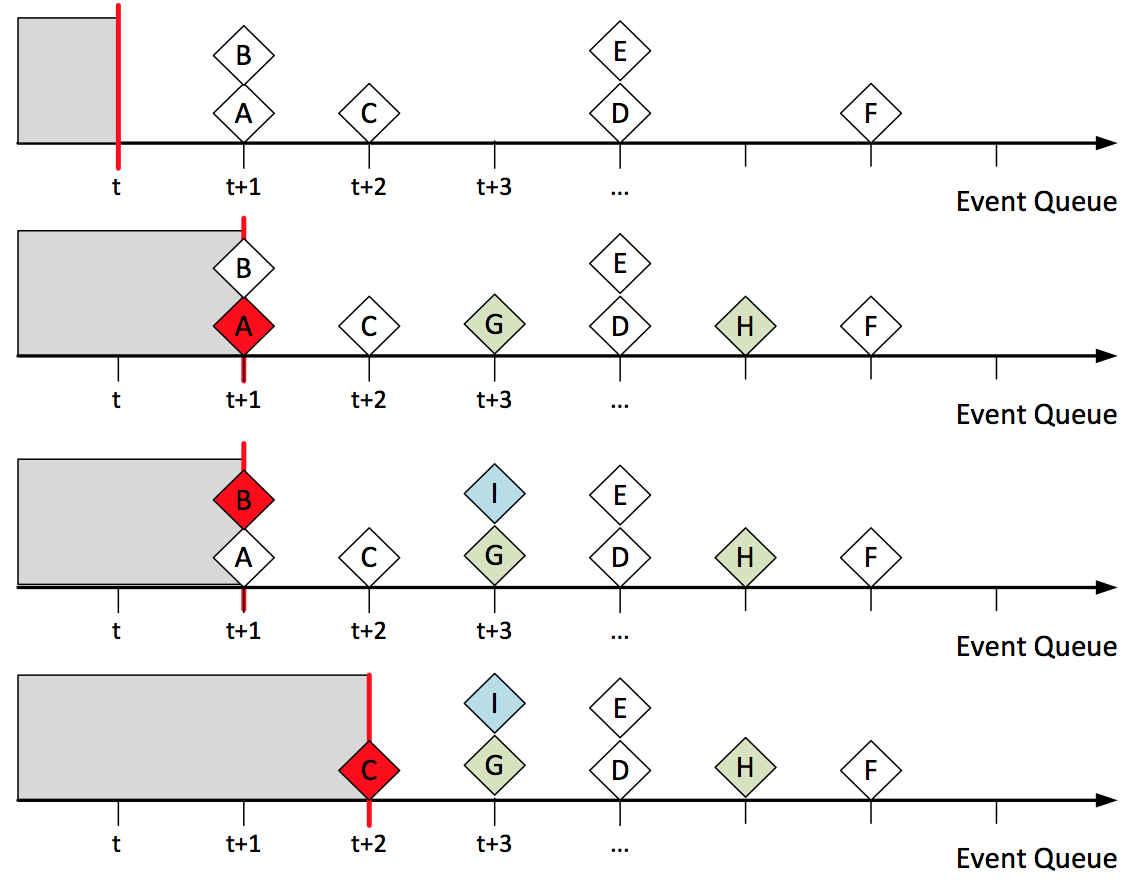
\includegraphics[width=\textwidth]{./bilder/EventQueue}
\end{minipage}

\begin{minipage}{0.4\textwidth}
	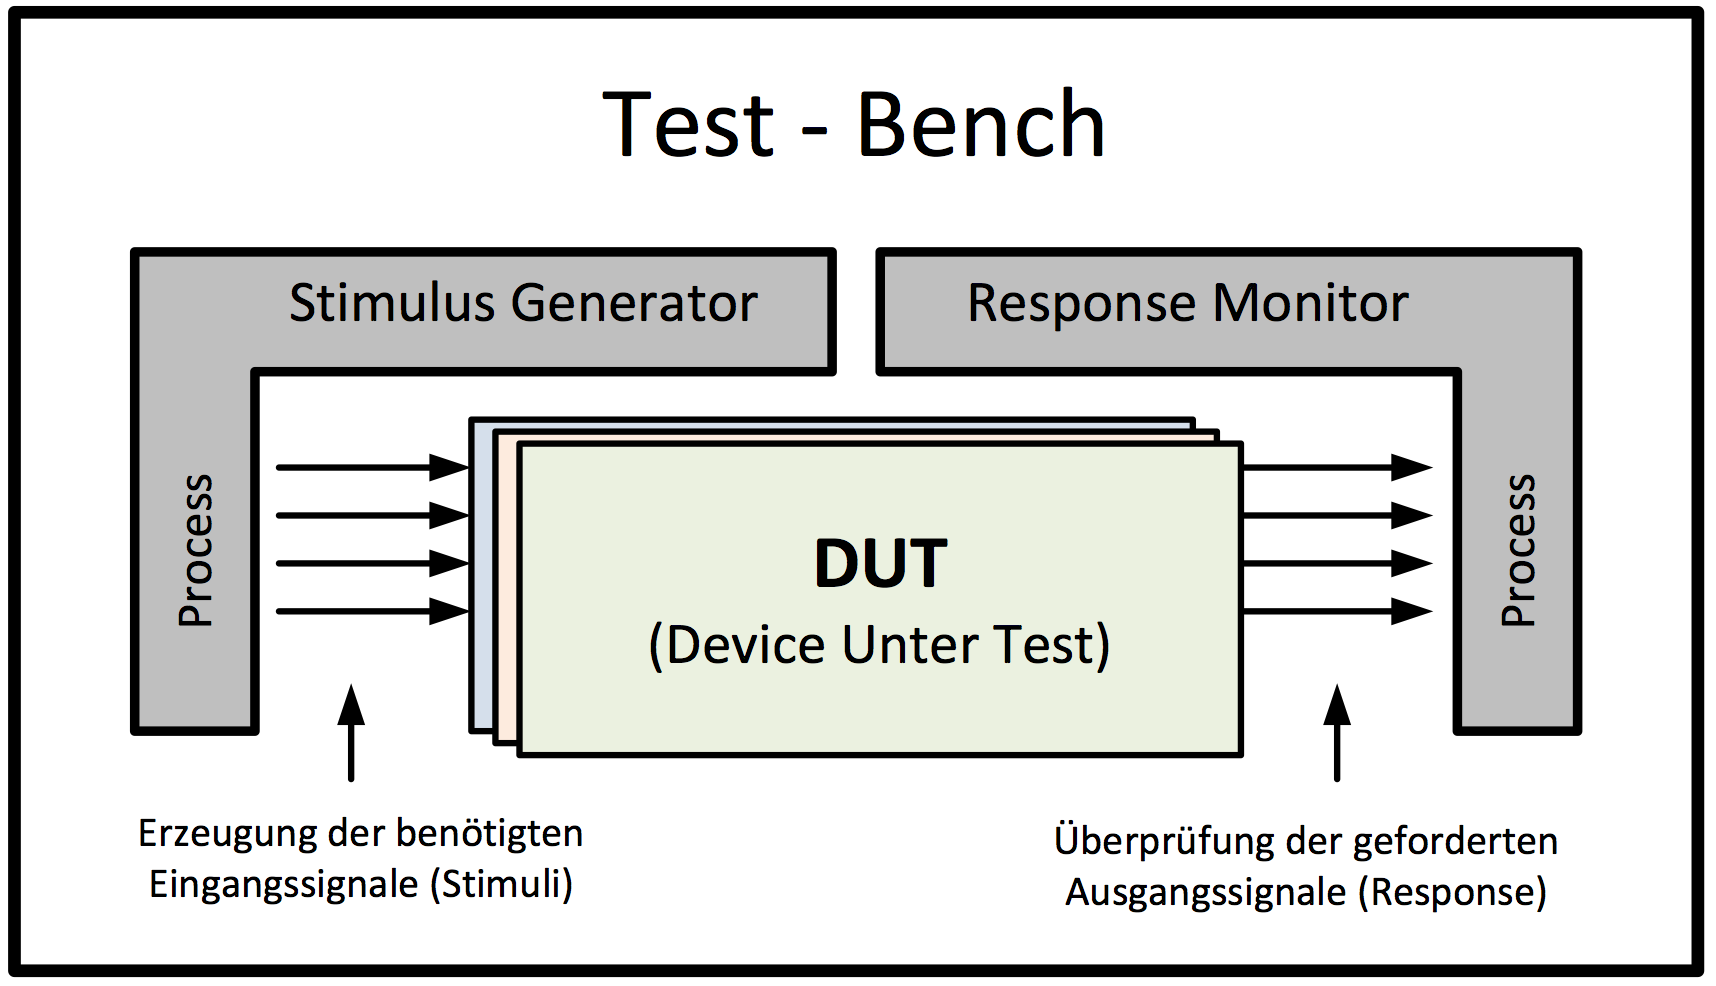
\includegraphics[width=\textwidth]{./bilder/TestBench}
\end{minipage}
\begin{minipage}{0.6\textwidth}
	\begin{tabular}{l}
		$\cdot$ In Test-Benchs werden oft Schleifen eingesetzt \\
		$\cdot$ Sie muss nicht Synthesefähig sein  \\
		$\cdot$ Automatische Überprüfung mit ASSERTs \\
		$\cdot$ Eine Test-Banch sollte eine leere entity haben {\tiny $\rightarrow$ keine Schnittstelle nach aussen}  \\
		$\cdot$ "`Simuli"' Eingang des DUT's, "`Respons"' erwartete Antwort\\
		$\cdot$ DUT "`1 zu 1"' aus work - library\\
	\end{tabular}
	
	\begin{minipage}{0.02\textwidth}
		\text{ } %platzhalter
	\end{minipage}
	\begin{minipage}{0.52\textwidth}
		\begin{VHDL}
-- for loop
[label:] for <parameter> in <range> loop
	{sequential statements}
end loop [label];
-- assert
[label:] assert condition [report string_expretion]
	[severity warning | error | ..];\end{VHDL}
	\end{minipage}
	\begin{minipage}{0.02\textwidth}
		\text{ } %platzhalter
	\end{minipage}
	\begin{minipage}{0.38\textwidth}
		\begin{VHDL}
-- Bsp fuer RST und CLK
rst <= '1', '0' after 150ms;
CLOCK : process
begin 
	clk <= '0';
	wait for (PERIOD / 2);
	clk <= '1';
	wait for (PERIOD / 2);
end process CLOCK;\end{VHDL}
	\end{minipage}
\end{minipage}



%%%%%%%%%%%%%%%%%%%%%%%%%%%%%%%%%%%%%%%%%%%%%%%%%%%%%%%%%%%%%%%%%%%%%%%%%%%%%%%%%%%%%%
% Key Concept V       
%%%%%%%%%%%%%%%%%%%%%%%%%%%%%%%%%%%%%%%%%%%%%%%%%%%%%%%%%%%%%%%%%%%%%%%%%%%%%%%%%%%%%%

\section{Key Concept V \tiny Parametisierbarkeit von Modellen}

\begin{minipage}{0.01\textwidth}
	\text{ } %platzhalter
\end{minipage}
\begin{minipage}{0.38\textwidth}

	Das Ziel von Parametern und Modellen ist es, dass man einen ähnlichen block wiederverwerten kann. z.B wenn man einen Zähler macht der auf 100 zählt, währe es schön wenn man den selben "`Block"' auch für einen der auf 230 zählt brauchen kann. 
	
	\begin{VHDL}
-- Entidy declaration mit generic Parameter:
entity entity_name is
    generic	({generic_name: type_name [:= default_value]}); 
	port  	(port_list);
end entity_name;

-- Component Declaration mit generic Parameter
component component_name
	generic	(generic_list);
	port	(port_list);
end component;
	\end{VHDL}
\end{minipage}
\begin{minipage}{0.02\textwidth}
	\text{ } %platzhalter
\end{minipage}
\begin{minipage}{0.58\textwidth}
	\begin{VHDL}
-- Zaehler Beispiel:
entity count_x is
	generic (max_count : integer := 127);
	port	(clk, rst, ena	: in std_logig;
			 oup			: out std_logic_vector
			 		(integer(ceil(log2(real(max_count)))) -1 downto 0));
end count_x

architecture RTL of count_x is 
	constant word_with: integer :=(integer(ceil(log2(real(max_count)))));
	signal present_count, next_count : unsigned(word_width-1 downto 0);
	
begin
	output_logic : oup <= std_logic_vector(present_count);	
	
	next_state_logic: process(present_count_ ena)
	begin
		next_count <= present_count;
		if ((present_count = max_cpunt) and (ena = '1')) then 
			next_count <= (others => '0');
		elsif (ena = '1') then next_count <= present_count + 1;
		end if;
	end process;
	-- Fortsetzung auf naechster Seite
\end{VHDL}
\end{minipage}

\begin{minipage}{0.01\textwidth}
	\text{ } %platzhalter
\end{minipage}
\begin{minipage}{0.38\textwidth}
	\begin{tabular}{l l}
		\multicolumn{2}{l}{\textbf{Fixierung von Designparameter}}  \\
		& \\
		Parameter zu Designzeit		& : Konstanten \\
		Parameter zu Compilezeit	& : Generic \\
		Parameter zu Laufzeit		& : Signale \\
	\end{tabular}
\end{minipage}
\begin{minipage}{0.02\textwidth}
	\text{ } %platzhalter
\end{minipage}
\begin{minipage}{0.58\textwidth}

	 \lstset{
	   	backgroundcolor=\color{grey},   % choose the background color
	     language=VHDL,			
	     basicstyle=\footnotesize\ttfamily,
	     breaklines=true,
	     frame=none,
	     columns=flexible,
	     keepspaces=true,
	     keywordstyle=\color{blue},
	     identifierstyle=\color{royalblue},
	     commentstyle=\color{green},
	     numbers=left,
	     numbersep=5pt,
	     numberstyle=\tiny\color{gray2},
	     rulecolor=\color{black}, 
	     stepnumber=1,
	     tabsize=4,
	     }

	\begin{lstlisting}[firstnumber=last]
-- Fortsetzung:
	register : process(clk, rst)
	begin 
		if (rst = '1') then present_count <= (others => '0');
		elsif (clk'event and (clk = '1')) then present_count <= next_count;
		end if;
	end process;
end architecture RTL;
\end{lstlisting}
\end{minipage}

%%%%%%%%%%%%%%%%%%%%%%%%%%%%%%%%%%%%%%%%%%%%%%%%%%%%%%%%%%%%%%%%%%%%%%%%%%%%%%%%%%%%%%
% Beispiele       
%%%%%%%%%%%%%%%%%%%%%%%%%%%%%%%%%%%%%%%%%%%%%%%%%%%%%%%%%%%%%%%%%%%%%%%%%%%%%%%%%%%%%%
\section{Beispiele}

 \lstset{
   	backgroundcolor=\color{grey},   % choose the background color
     language=VHDL,			
     basicstyle=\footnotesize\ttfamily,
     breaklines=true,
     frame=none,
     columns=flexible,
     keepspaces=true,
     keywordstyle=\color{blue},
     identifierstyle=\color{royalblue},
     commentstyle=\color{green},
     numbers=left,
     numbersep=5pt,
     numberstyle=\tiny\color{gray2},
     rulecolor=\color{black}, 
     stepnumber=1,
     tabsize=4,
     }

\begin{minipage}{0.01\textwidth}
	\text{ } %platzhalter
\end{minipage}
\begin{minipage}{0.48\textwidth}
	\begin{lstlisting}
library ieee;
use ieee.std_logic_1164.all;
use ieee.math_real.all;

entity edgedetpos_random_tb is
end edgedetpos_random_tb;

architecture tb of edgedetpos_random_tb is
	constant f : integer := 1000;       -- Frequency in HZ
	constant T : time    := 1 sec / f;

	component edgedetpos
		port(
			clk  : in  std_ulogic;
			nrst : in  std_ulogic;
			inp  : in  std_ulogic;
			oup  : out std_ulogic
		);
	end component;

	for all : edgedetpos use entity work.edgedetpos(behavioral);

	signal clk_tb     : std_ulogic;
	signal nrst_tb    : std_ulogic;
	signal inp_tb     : std_ulogic;
	signal oup_tb     : std_ulogic;
	signal oup_exp_tb : std_ulogic;

begin
	dut : edgedetpos
		port map(
			clk  => clk_tb,
			nrst => nrst_tb,
			inp  => inp_tb,
			oup  => oup_tb
		);

	stimuli_clk : process
	begin
		clk_tb <= '0';
		wait for T / 2;
		clk_tb <= '1';
		wait for T / 2;
	end process;

	stimuli_nrst : nrst_tb <= '0', '1' after 3 ms;
	
	stimuli_inp : process
		variable t      : time;
		variable t_real : real;
		variable seed1  : positive := 1;
		variable seed2  : positive := 1;	
	\end{lstlisting}
\end{minipage}
\begin{minipage}{0.02\textwidth}
	\text{ } %platzhalter
\end{minipage}
\begin{minipage}{0.48\textwidth}
	\begin{lstlisting}[firstnumber=last]
	begin
		inp_tb <= '0';
		loop
			UNIFORM(seed1, seed2, t_real);
			t := (t_real * 0.007) * 1 sec;
			wait for t;
			inp_tb <= not inp_tb;
		end loop;
	end process;
	
stimuli_oup_exp : process
	begin
		loop
			oup_exp_tb <= '0';
			if (nrst_tb = '0') then
				wait until (nrst_tb'event and nrst_tb = '1');
				wait until (clk_tb'event and clk_tb = '1');
			end if;
			if (inp_tb = '0') then
				while (inp_tb = '0') loop
					wait until (clk_tb'event and clk_tb='1');
				end loop;
				oup_exp_tb <= '1';
				wait until (clk_tb'event and clk_tb = '1');
				oup_exp_tb <= '0';
			else
				wait until (clk_tb'event and clk_tb = '1');
			end if;
		end loop;
		wait;
	end process;

	evaluation : process
	begin
		wait until (clk_tb'event and clk_tb = '1');
		wait for 0.5 us;
		loop
			assert (oup_exp_tb = oup_tb) report "Error oup" severity error;
			wait for 1 us;
		end loop;
		wait;
	end process;

end tb;








	\end{lstlisting}
\end{minipage}

\begin{minipage}{0.01\textwidth}
	\text{ } %platzhalter
\end{minipage}
\begin{minipage}{0.48\textwidth}
	\begin{lstlisting}
library ieee;
use ieee.std_logic_1164.all;

entity edgedetpos is
	port(
		clk  : in  std_ulogic;
		nrst : in  std_ulogic;
		inp  : in  std_ulogic;
		oup  : out std_ulogic
	);
end;

architecture behavioral of edgedetpos is
	type state_type is (resetstate, wait_for_1, pulse, wait_for_0);

	signal present_state : state_type;
	signal next_state    : state_type;

begin
	-- short form for output logic. Code version with process: see edgedetneg
	Output_logic:	oup <= '1' when present_state = pulse else '0';

	Next_state_logic : process(inp, present_state)
	begin
		next_state <= wait_for_0;       -- default state
		case present_state is
			when wait_for_1 =>
				if (inp = '1') then
					next_state <= pulse;
				else
					next_state <= wait_for_1;
				end if;
			when pulse =>
				if (inp = '0') then
					next_state <= wait_for_1;
				-- else						-- due to default
				-- next_state <= wait_for_0;
				end if;
			when wait_for_0 =>
				if (inp = '0') then
					next_state <= wait_for_1;
				-- else
				-- next_state <= wait_for_0;
				end if;
			when others =>
				if (inp = '0') then
					next_state <= wait_for_1;
				-- else
				-- next_state <= wait_for_0;
				end if;
		end case;
	end process;

	registers : process(nrst, clk)
	begin
		if (nrst = '0') then
			present_state <= resetstate;
		elsif (clk = '1') and clk'event then
			present_state <= next_state;
		end if;
	end process;

end behavioral;
	\end{lstlisting}
	\begin{lstlisting}
entity BUS_DRIVER is
port(
	sel: 		in std_ulogic;
	data_out: 	in std_ulogic_vector(7 downto 0);
	my_bus: 	inout std_logic_vector(7 downto 0);
	data_in: 	out std_ulogic_vector(7 downto 0));
end BUS_DRIVER;
	\end{lstlisting}
\end{minipage}
\begin{minipage}{0.02\textwidth}
	\text{ } %platzhalter
\end{minipage}
\begin{minipage}{0.48\textwidth}
	\begin{lstlisting}[firstnumber=last]
architecture TEST of BUS_DRIVER is

begin
    
-- Bus_Komponente
	READ: data_in <= to_stdulogicVector(my_bus);
	WRITE: process(sel, data_out)
		begin
			if sel = '1' then my_bus <= To_StdLogicVector(data_out);
			else my_bus <= 	(others => 'Z');
		end if;
	end process WRITE;

end Test;	
	\end{lstlisting}
	\begin{lstlisting}
entity mux3x8_top is
	port(
		sel  : in  bit_vector(1 downto 0);
		inp0 : in  bit_vector(7 downto 0);
		inp1 : in  bit_vector(7 downto 0);
		inp2 : in  bit_vector(7 downto 0);
		oup  : out bit_vector(7 downto 0));
end mux3x8_top;

architecture RTL of mux3x8_top is
	component mux3x8
		port(sel  : in  bit_vector(1 downto 0);
			 inp0 : in  bit_vector(7 downto 0);
			 inp1 : in  bit_vector(7 downto 0);
			 inp2 : in  bit_vector(7 downto 0);
			 oup  : out bit_vector(7 downto 0));
	end component mux3x8;

	for all: mux3x8 use entity work.mux3x8(PROCESS_IF_NO_Default); 
begin
	 U1: mux3x8
	 	port map(sel  => sel,
	 		     inp0 => inp0,
	 		     inp1 => inp1,
	 		     inp2 => inp2,
	 		     oup  => oup);
end architecture RTL;	
	\end{lstlisting}
	\begin{lstlisting}
entity or2 is
  port(
    a, b : in bit;
    y : out bit);
  end;

architecture behavioral of or2 is
begin
   y <= a or b;
end behavioral;
	\end{lstlisting}
	\begin{lstlisting}
-- Beispiel ENUM ENCODING
type STATE_TYPE is (ST_NORMAL, ST_HSET, ST_MSET, ST_SSYNC);
-- Explizite codierung mit ENUM_ENCODING
attribute ENUM_ENCODING: STRING;
attribute ENUM_ENCODING of STATE_TYPE:
	type is "0001 0010 0100 1000"; -- one hot
signal PRESENT_State, NEXT_State : STATE_TYPE;

				--------------------------
				-- State     | Encoding --
				-------------|------------
				-- st_normal | 0001     --
				-- st_hset   | 0010     --
				-- st_mset   | 0100     --
				-- st_ssync  | 1000     --
				--------------------------
	\end{lstlisting}
\end{minipage}






\end{document}
